\documentclass[conference]{IEEEtran}
\usepackage{times}

% numbers option provides compact numerical references in the text. 
\usepackage[numbers]{natbib}
\usepackage{multicol}
\usepackage[bookmarks=true]{hyperref}


\usepackage{booktabs}
\usepackage{float}
\usepackage{graphicx}
\usepackage{amsfonts}
\usepackage{bbding}
\usepackage{multirow}
\usepackage{makecell}
\usepackage{caption}
\usepackage{amsmath}
\usepackage{xcolor}

\newcommand{\specialcell}[2][c]{%
  \begin{tabular}[#1]{@{}c@{}}#2\end{tabular}}
  
\newcommand{\authnote}[2]{$\ll$\textsf{\footnotesize #其他问题 #2}$\gg$}
%\newcommand{\authnote}[2]{}

\newcommand{\chuan}[1]{{\color{蓝色}\authnote{}{#1}}}
\newcommand{\xingyu}[1]{{\color{红色}\authnote{兴}{#1}}}


\pdfinfo{
   标题:我们的新主宰者/创建日期 (D:20101201120000) /主题 (机器人) /关键字 (机器人;主宰者)
}

\usepackage{xeCJK}
\setCJKmainfont{Noto Serif CJK SC}
\begin{document}

% paper title
\title{策略学习的任意点轨迹建模}

% You will get a Paper-ID when submitting a pdf file to the conference system
% \author{Author Names Omitted for Anonymous Review. Paper-ID [63]}
\author{文 $^{*1,2,5}$ \quad 兴林$^{*1}$ \quad 约翰·索$^{*3}$ \\
凯陈$^{6}$ \quad 道$^{6}$ \quad 高$^{2,4,5}$ \quad 皮埃特·阿贝尔$^{1}$ \\
$^{1}$美国大学伯克利大学 \quad $^{2}$华大学的IIIS \quad $^{3}$斯坦福大学 \\
$^{4}$上海人工智能实验室 \quad $^{5}$城学会 \quad $^{6}$ 子 \\
}

%\author{\authorblockN{Michael Shell}
%\authorblockA{School of Electrical and\\Computer Engineering\\
%Georgia Institute of Technology\\
%Atlanta, Georgia 30332--0250\\
%Email: mshell@ece.gatech.edu}
%\and
%\authorblockN{Homer Simpson}
%\authorblockA{Twentieth Century Fox\\
%Springfield, USA\\
%Email: homer@thesimpsons.com}
%\and
%\authorblockN{James Kirk\\ and Montgomery Scott}
%\authorblockA{Starfleet Academy\\
%San Francisco, California 96678-2391\\
%Telephone: (800) 555--1212\\
%Fax: (888) 555--1212}}


% avoiding spaces at the end of the author lines is not a problem with
% conference papers because we don't use \thanks or \IEEEmembership


% for over three affiliations, or if they all won't fit within the width
% of the page, use this alternative format:
% 
%\author{\authorblockN{Michael Shell\authorrefmark{1},
%Homer Simpson\authorrefmark{2},
%James Kirk\authorrefmark{3}, 
%Montgomery Scott\authorrefmark{3} and
%Eldon Tyrell\authorrefmark{4}}
%\authorblockA{\authorrefmark{1}School of Electrical and Computer Engineering\\
%Georgia Institute of Technology,
%Atlanta, Georgia 30332--0250\\ Email: mshell@ece.gatech.edu}
%\authorblockA{\authorrefmark{2}Twentieth Century Fox, Springfield, USA\\
%Email: homer@thesimpsons.com}
%\authorblockA{\authorrefmark{3}Starfleet Academy, San Francisco, California 96678-2391\\
%Telephone: (800) 555--1212, Fax: (888) 555--1212}
%\authorblockA{\authorrefmark{4}Tyrell Inc., 123 Replicant Street, Los Angeles, California 90210--4321}}



\twocolumn[{%
\renewcommand\twocolumn[1][]{#1}%
\maketitle
\begin{center}
    \centering
    \captionsetup{类型=图}
    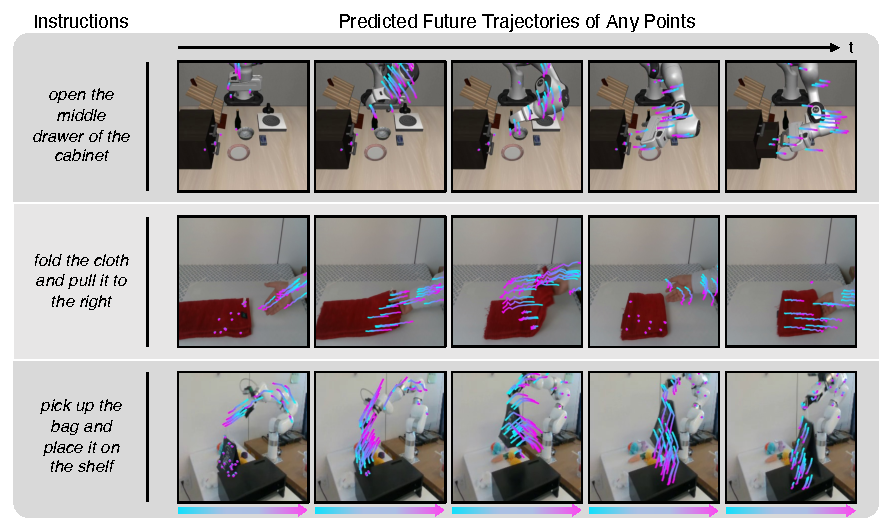
\includegraphics[width=0.92\textwidth]{fig/pull.pdf}
    \captionof{图表}{根据任务指令和图像框架中的任何点的初始位置,我们的任意点轨迹模型 (ATM) 可以预测这些点的未来轨迹,以条件完成任务. 在训练模型后,预测轨迹作为学习视觉动力策略的有效指导,用于一组语言条件操作任务.}
\end{center}%
}]

\IEEEpeerreviewmaketitle

\makeatletter\def\Hy警告#1{}\makeatother\let\thefootnote\relax\footnotetext{*第一三位作者也同样做了贡献:文领导了实施和实验.兴林提出了这个想法,监督了技术开发,并为模型调试做了贡献.约翰·索实施了机器人到机器人转移实验和UniPi基线.}

\begin{abstract}
演示学习是教机器人新技能的强大方法,并且拥有更多演示数据往往会改善策略学习.然而,收集演示数据的高成本是显著的瓶.视频作为丰富的数据来源,包含行为,物理和语义知识,但由于缺乏动作标签而从它们中提取特定控制信息是个挑战. 在本工作中,我们引入了一个新框架,即Any-point Trajectory Modeling (ATM),通过预训练轨道模型来利用视频演示来预测视频框架内的任意点的未来轨道.一旦训练,这些轨道提供了详细的控制指导,使得使用视觉标签数据学习强大的策略.在我们在模拟和现实世界中评估的超过130个语言条件任务中,ATM超过了强大的视频预训基线的80$\%$ 另外,我们还显示了从人类视频和不同机器人形态的视频中有效地转移操纵技能. 视觉化和代码可在: \url{https://xingyu-lin.github.io/atm}.
\end{abstract}    
\section{引言} \label{sec:intro}
近年来,计算机视觉和自然语言理解取得了显著进展~\cite{kirillov2023segment,brown2020language}机器人技术,扩大人类示范数据是学习新技能的关键.~\cite{brohan2022rt,padalkar2023open,fang2023rh20t}随着较大的数据集的提高,~\cite{mandlekar2021matters,brohan2022rt}然而,通过远程操作设备收集的人类示范,通常是以动作标签的轨迹~\cite{zhang2018deep,wu2023gello}收集需要时间和劳动力. $130K$ 轨迹~\cite{brohan2022rt} 收集数据成为机器人学习的一个重大瓶.

视频包含有关行为,物理和语义学的知识,呈现出另一个数据来源. 然而,缺乏动作标签使得利用视频数据在策略学习中很难.之前的研究已经通过使用视频预训的自我监督目标来解决这一问题,以学习观察的特征表示策略学习~\cite{sermanet2018tcn,nair2023r3m,seo2022reinforcement}然而,一个特征表示只描述当前的时间阶段的状态,大大忽略了预测未来状态的过渡动态.为了明确地模拟过渡动态,之前的研究已经开发出了预测视频模型,预测未来的图像框架从当前的模型来指导策略学习~\cite{du2023unipi,yang2023learning, Escontrela23arXiv_VIPER}然而,学习视频预测模型来控制引入两个挑战.第一,视频预测任务通过模型每一个像素的变化来避免任何抽象性,将物理运动与纹理和照明等视觉外观相结合.这种结合使得模型难以进行,通常导致幻觉和不现实的未来预测~\cite{du2023unipi}由于这些模型在训练和推理方面都具有计算要求.由于计算资源有限,性能显著下降.~\cite{du2023unipi,black2023zero}由于这些策略的强制性,

在本文中,我们提出了一个新型和结构化的表现,以桥接视频预训和策略学习.我们首先将每个状态表现为视频框架中的一组点.~通过电子图像,我们可以将光谱测试到图像中,并将它们的位置视为输入,并将它们的未来轨迹输出.我们预测这些轨迹在摄像头坐标框架中以最大限度地减少校准摄像头的假设.这些2D点轨迹与3D空间中的粒子轨迹相符,并且是可以转移到不同的领域和任务的运动的普遍表示.与视频预测方法相比,基于粒子的轨迹建模提供了对物理动态的忠实抽象,自然包含了像物体永久性和连续运动这样的诱导偏见.我们首先在无动作视频数据集上预训了轨迹模型. 预测的轨迹可以作为指导控制策略的子目标.我们然后使用最小的动作标签示范数据训练轨迹指导的策略.~\cite{karaev2023cotracker}在我们在模拟和现实世界中评估的超过130项语言条件任务中,ATM在视频预训方面明显超过了各种强的基线,实现了平均成功率的 $63\%$ 与最高的成功率相比 $37\%$ 通过以前的方法, 标志着改善 $80\%$另外,我们还证明了我们的方法能够从人类视频和不同形态的机器人视频中有效地转移学习.
\begin{enumerate}
  \item 我们提出了任意点轨迹模型,这是一个简单而新鲜的框架,
  \item 通过对模拟基准和现实世界进行广泛的实验,我们证明了我们的方法可以有效地利用预训练中的视频数据,并在模拟学习环境中显著优于各种视频预训基线.
  \item 我们通过跨体体视频展示了有效的学习.
\end{enumerate}

\section{相关工作}
在学习端到端视觉动力策略中,该策略通常被定义为一个神经网络,将图像观测作为输入表示~\cite{reed2022generalist,brohan2022rt,walke2023bridgedata}由于缺乏诱导偏见,这些方法需要对大量的示范轨迹进行培训,而收集成本昂贵.~\cite{qin2020keto,manuelli2020keypoints}网格~\cite{lin2021VCD,huang2022medor}通过神经3D表示~\cite{li20213d,rashid2023language}尽管如此,以前的结构通常限制了策略的具体任务.相反,我们建议利用图像中的任意点的未来轨迹作为策略的额外输入,对任务和环境做出最小的假设.我们展示了其广泛应用到超过130个语言条件的操作任务.在导航和运输中,通常构建由机器人的未来轨迹指导的策略.~\cite{aguiar2007trajectory,peng2018deepmimic}在操纵中,一些作品探讨了基于流量的指导~\cite{goyal2022ifor,seita2023toolflownet,gu2023rt}之前的研究只追踪了特定任务的点,例如机器人的终极效应或人类的手. \citet{vecerik2023robotap} 设计选择需要更多的仪器,如分分任务成多个阶段,预测每个阶段的目标位置,并运行追踪器在推断时间.相反,我们提出了一个更简单的框架,使其在更多种设置中应用.

视频预训练用于控制.视频包含有关行为和动态的丰富信息,这可以帮助学习策略.然而,视频预训练仍然是由于缺乏动作标签而具有挑战性.一行作品首先学习了反动力学模型,该模型从两个邻近的框架预测到行动,然后将视频标签为伪行动~\cite{schmeckpeper2019learning, baker2022vpt, torabi2018behavioral,schmidt2024learning}尽管如此,反动力学模型通常是在有限的动作标签数据集上训练,并且不很好地概括,特别是在连续行动中.~\cite{sermanet2017tcn,nair2023r3m,ma2023vip}视频预测学习作为预训已经显示出了有前途的结果.~\cite{du2023unipi,Ko2023Learning,bharadhwaj2023zero,yang2023learning,Escontrela23arXiv_VIPER}在策略学习过程中,使用视频预测模型生成未来的子目标,然后可以学习目标条件的策略,以达到子目标.然而,视频预测模型往往导致幻觉和不现实的物理运动.此外,视频模型需要广泛的计算,这是一个问题,特别是在推断时间.相反,我们的方法模型点的轨迹,自然包含像对象永久性的诱导偏见,同时需要更少的计算.这使我们的轨迹模型在策略执行过程中能够运行闭环.此外,轨迹为策略提供密集的指导,作为一个前进的运动.

特别有趣的是,许多先前的著作提出了从人类视频的丰富来源中学习的建议.~\cite{xiong2021learning,shao2021concept2robot, mendonca2023structured,bahl418affordances,shaw2023videodex,wang2023mimicplay}然而,这些作品往往明确从人类视频中提取手姿势或接触区域,从而损失了其余物体动态的信息. 相比之下,我们的方法模拟了任意点的轨迹,可以从人类视频和不同机器人的视频中学习.
\begin{figure*}
    \centering
  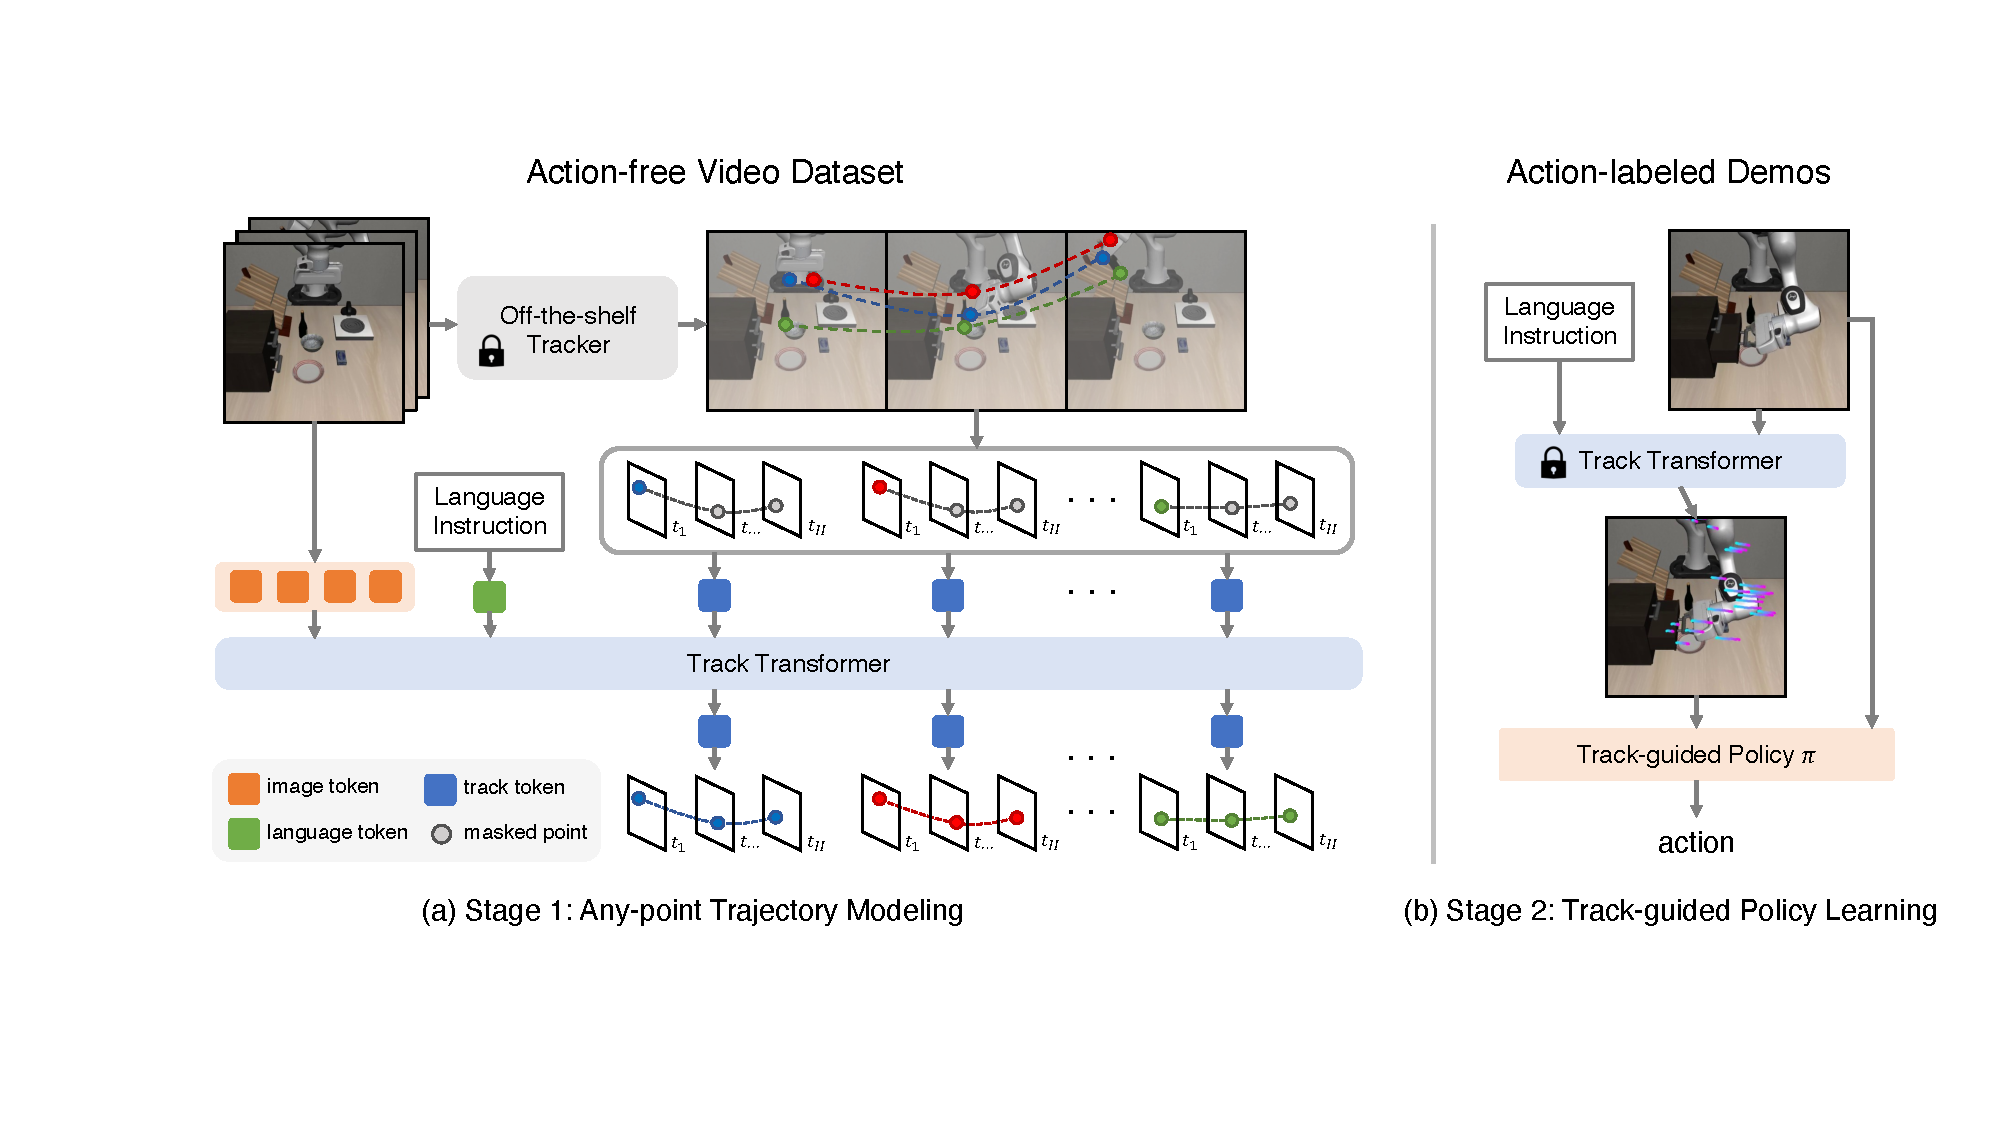
\includegraphics[width=\linewidth]{fig/system.pdf}
  \caption{根据我们所做的操作,我们将在视频中进行测试,并将视频的数据集进行测试. (a) 在第一阶段,由于无动作视频数据集,我们首先在一个视频框架上采样2D点,并使用预训练的跟踪器跟踪视频中它们的轨迹.然后我们训练了轨迹 Transformer,以根据当前的图像观测,语言指令和点的初始位置预测未来点轨迹.对于变压器输入,我们将未来的点位置取代为掩盖值. (2) 在第二阶段,我们学习了测试指导的策略,以预测控制行动.预测的轨道的指导使我们能够从仅少数操作标签的示范中学习强大的策略. }
  \label{fig:system}
\end{figure*}


\section{预期} \label{sec:prelim}
在本文中,我们将从一小组以行动标记的示范轨迹中学习强大的控制策略. 我们的核心目标是利用更可扩展,未标记的视频作为预训的数据来源. 

 首先,我们将无动作视频数据集表示为 $\mathcal{T}_{o}=\{(\tau_o^{(i)}, \ell^{(i)})\}_{i=1}^{N_{o}},$ 在哪里 $\ell^{(i)}$ 是为 语言教学 $i^{th}$ 事件和 $\tau_o^{(i)} = \{o_t^{(i)}\}_{t=1}^T$ 仅仅是观测轨迹,由摄像头图像组成. $\mathcal{T}_{a}=\{(\tau_a^{(i)}, \ell^{(i)})\}_{i=1}^{N_{a}},$ 在哪里 $\tau_a^{(i)} = \{o_t^{(i)}, a_t^{(i)}\}_{t=1}^T$ 在模仿学习过程中,我们的目标是学习一种策略 $\pi_{\theta}$参数为 $\theta$ 通过以下行为克隆目标模仿专家行为:
\begin{equation}
    \pi_{\theta}^{*} = \arg\min_{\theta} E_{(o_t,a_t, \ell)\sim \mathcal{T}_{a}}\Big[\mathcal{L}\Big(\pi_{\theta}(o_t, \ell), a_t\Big)\Big],
    \label{eq:bc}
\end{equation}
在哪里 $\mathcal{L}$ 输出值的值是输出值的值.

 视频跟踪近期的进步~\cite{harley2022particle, doersch2023tapvid, doersch2023tapir, wang2023tracking, zheng2023pointodyssey} 通过电子视频,我们可以在视频框架中跟踪每个点的轨迹,而无需外部监督.~\cite{karaev2023cotracker}根据视频的图像序列, $o_1, ..., o_T$任何时间步骤 $\bar{t} \in [1, T]$并且在这个框架中设置了一组点 $\{p_{\bar{t}, k}\}_{k=1}^{K}$在哪里 $p_{\bar{t}, k} = (x, y)$ 监测任务是预测每个图像中的相应点的2D相机图像坐标 $p_{t, k}$ 在哪里 $t =1 \dots T$在本文中,我们用轨迹和跟踪术语交换地指指任何点的二维坐标序列, $(p_1, \dots, p_T)$我们只在摄像头框架中模拟2D轨迹,以便我们不需要对多视图摄像头做出额外的假设,或者可用深度,从而允许未来扩展到更多种视频数据集. $v_{t, k}$ 标示点是否被步骤遮蔽 $t$.

\section{方法}
视频包含了大量关于世界的先前信息, 捕捉了物理动态,人类行为和语义,~\cite{sermanet2017tcn,nair2023r3m,ma2023vip}通过视频,我们将学习一个模型,以预测未来状态,以指导控制策略.通过这种方式,我们可以基本上分解视觉运动策略学习挑战成两个部分.第一部分是学习如何通过生成未来状态作为具体的子目标,这仅仅是从视频中学习.第二部分是学习预测控制行动来遵循子目标,这些行动需要比学习策略的数据少得多.~\cite{du2023unipi,Ko2023Learning,black2023zero} 视频预测在培训和推断阶段都需要资源,但其重点重建像素级细节,这些细节往往是策略学习的外在,可能会对后续策略学习的效率产生不利影响.

我们提出任意点轨迹建模~图所示,~\ref{fig:system}, 
% ATM learns to predict future point trajectories in a video frame as the pre-training, then uses the predicted trajectories to guide policy learning. 
预测系统是一个两阶段的框架:首先学习在视频框架中预测未来的点轨迹,作为预训,使用大规模无动作视频,然后使用预测轨迹来指导策略学习,使用少数拍摄的动作标签演示. 我们的建议方法将在本节详细介绍:~\ref{sec:track-model}首先,我们将描述如何从无动作视频数据集中学习一个点轨迹预测模型 $\mathcal{T}_{o}$然后在Sec.~\ref{sec:track-policy}我们将概述如何利用预训轨道预测模型来从有限的行动标记轨道数据集中学习轨迹引导的策略 $\mathcal{T}_a$.

\subsection{从视频数据集进行轨迹建模} \label{sec:track-model}
我们的目标是预先训练一个视频模型,预测未来的点轨迹. $o_t$ 在时间步骤下 $t$图像框架上的任何2D查询点 $\mathbf{p}_t = \{p_{t, k}\}_{k=1}^K$语言教学 $\ell$我们学习一个模型. $\mathbf{p}_{t:t+H} = \tau_\theta(o_t, \mathbf{p}_t, \ell)$ 预测未来查询点的坐标 $H$ 摄像机框架中的步骤,  $\mathbf{p}_{t:t+H} \in \mathbb{R}^{H \times K \times 2}$为了模拟轨道,我们提出了轨迹 Transformer,~\ref{fig:system} (a).

\paragraph{单独监督的轨道注释.} \label{sec:TAP-annotation}
首先,我们从无动作视频生成点轨迹,~\ref{sec:prelim}视频的预处理,并生成一个追踪数据集. $\bar{t}$ 随机样本的位置在这个框架上,并通过运行跟踪器生成他们的轨迹.然而,对于静态相机,大多数随机样本的点将在后台,因此在训练我们的轨迹 Transformer时提供很少的信息. $n~\times~n$ 在框架上 $\bar{t}$ 视频中所有的点格格,以获得最初的轨道集 $\tau \in \mathbb{R}^{n^2 \times T \times 2}$随后,我们通过对时间的差异进行选,在视频中未移动的点,在最后一步中,我们重新样本了选位置的点,最后使用跟踪器生成它们的位置.

\paragraph{模拟多动轨道.}
我们将未来预测问题正式化为一个多模式的掩盖预测问题:我们旨在预测每个点的未来位置,根据其当前位置,当前的图像观察和任务的语言指示.我们首先将不同的模式编码到共享嵌入空间中,每个模式由几个代币表示.对于轨道,我们在编码之前掩盖所有点的未来位置,然后单独编码每个点成一个代币.~\cite{devlin2019-bert} 对于图像,我们将它们分为图像补丁, $50\%$ 接下来我们通过一个大型变压器模型传递所有代币.最后,我们将跟踪代币解码成相应点的未来轨迹.~\citet{he2022masked} 通过这个预训练过程,我们的轨迹 Transformer学习了视频框架内的粒子的前进运动.


\subsection{基于轨迹引导的策略学习}\label{sec:track-policy}
训练后,我们可以根据观察预测未来轨道的轨迹 Transformer,

\paragraph{随意追踪点.} 在轨迹 Transformer预训练中,我们可以在没有大动作的情况下过轨道.然而,使用这种论学需要知道每个点的未来位置,这在策略推断过程中计算可能昂贵.相反,我们认为仅仅仅使用一个固定的32点在网格上来进行策略.这种样本采集方法避免了学习关键点或找到跟踪点的潜在复杂性~\cite{vecerik2023robotap} 作为一个基本的方法,我们可以使用一个不同的点样本方案,

\begin{figure}[ht]
  \centering
  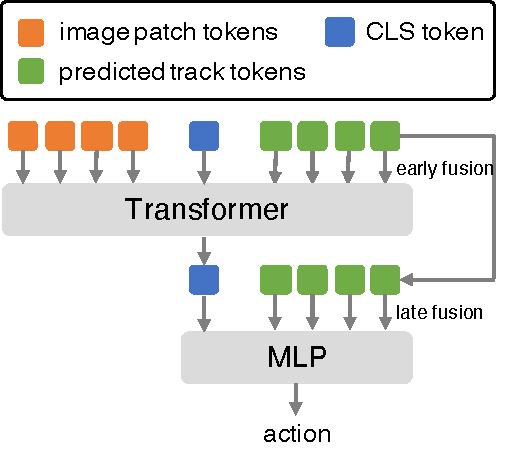
\includegraphics[width=.75\linewidth]{fig/simplified_track_policy.pdf}
  \caption{鉴于目前的观察和预测的轨迹 Transformer的预测,我们从有限的示范数据集中训练了轨迹引导的策略.}
  \label{fig:track_policy}  
\end{figure}


\paragraph{基于轨迹引导的策略学习.} 遵循轨道的策略 $\pi(a_t | o_t, p_{t:t+H})$ 接收了当前的观察 $o_t$ 预测的轨迹 $p_{t:t+H}$ 简单的说明是我们的策略架构.~\ref{fig:track_policy}我们的变革策略架构遵循以前的建筑~\cite{liu2023libero, kim2021vilt}虽然预测的轨道本身已经提供了丰富的信息来预测行动,但我们仍然将文本图像观测纳入我们的策略,以便没有信息丢失,~\cite{lin2023spawnnet}预测:我们将轨道代币与图像代币 (早期融合和后期融合) 结合起来,以确保轨道的指导信息可以有效地集成.令人惊的是,由于轨道已经提供了细微的子目标,我们发现该策略不再需要语言指导作为任务规范.基本上,提供的轨道将难以学习的难题降低到更容易的子目标后的问题,将该策略降低到反动动态模型.我们的轨迹引导策略是训练的MSE损失.请注意,我们的策略模型的重量是随机初始化而不是像其他视频训练方法一样从预训练的轨迹 Transformer中复制.~\cite{nair2023r3m,ma2023vip}由于有针对性,该项目将在" 预测轨迹"中进行单独研究.


\section{实验}\label{sec:experiment}
我们进行了实验,以回答以下问题:
\begin{itemize}
    \item 如何与无动作视频学习的先进视频预训和行为克隆基线相比较?
    \item 通过电子视频数据学习,可以使用ATM吗?
\end{itemize}
我们的实验分为三部分.~\ref{sec:video_bc}在"电子游戏"中,我们将ATM与视频预训基线进行比较,~\ref{sec:human_video}通过电子设备,我们可以通过人类视频进行有效学习.~\ref{sec:ablation}.

\begin{figure*}[ht]
    \centering
    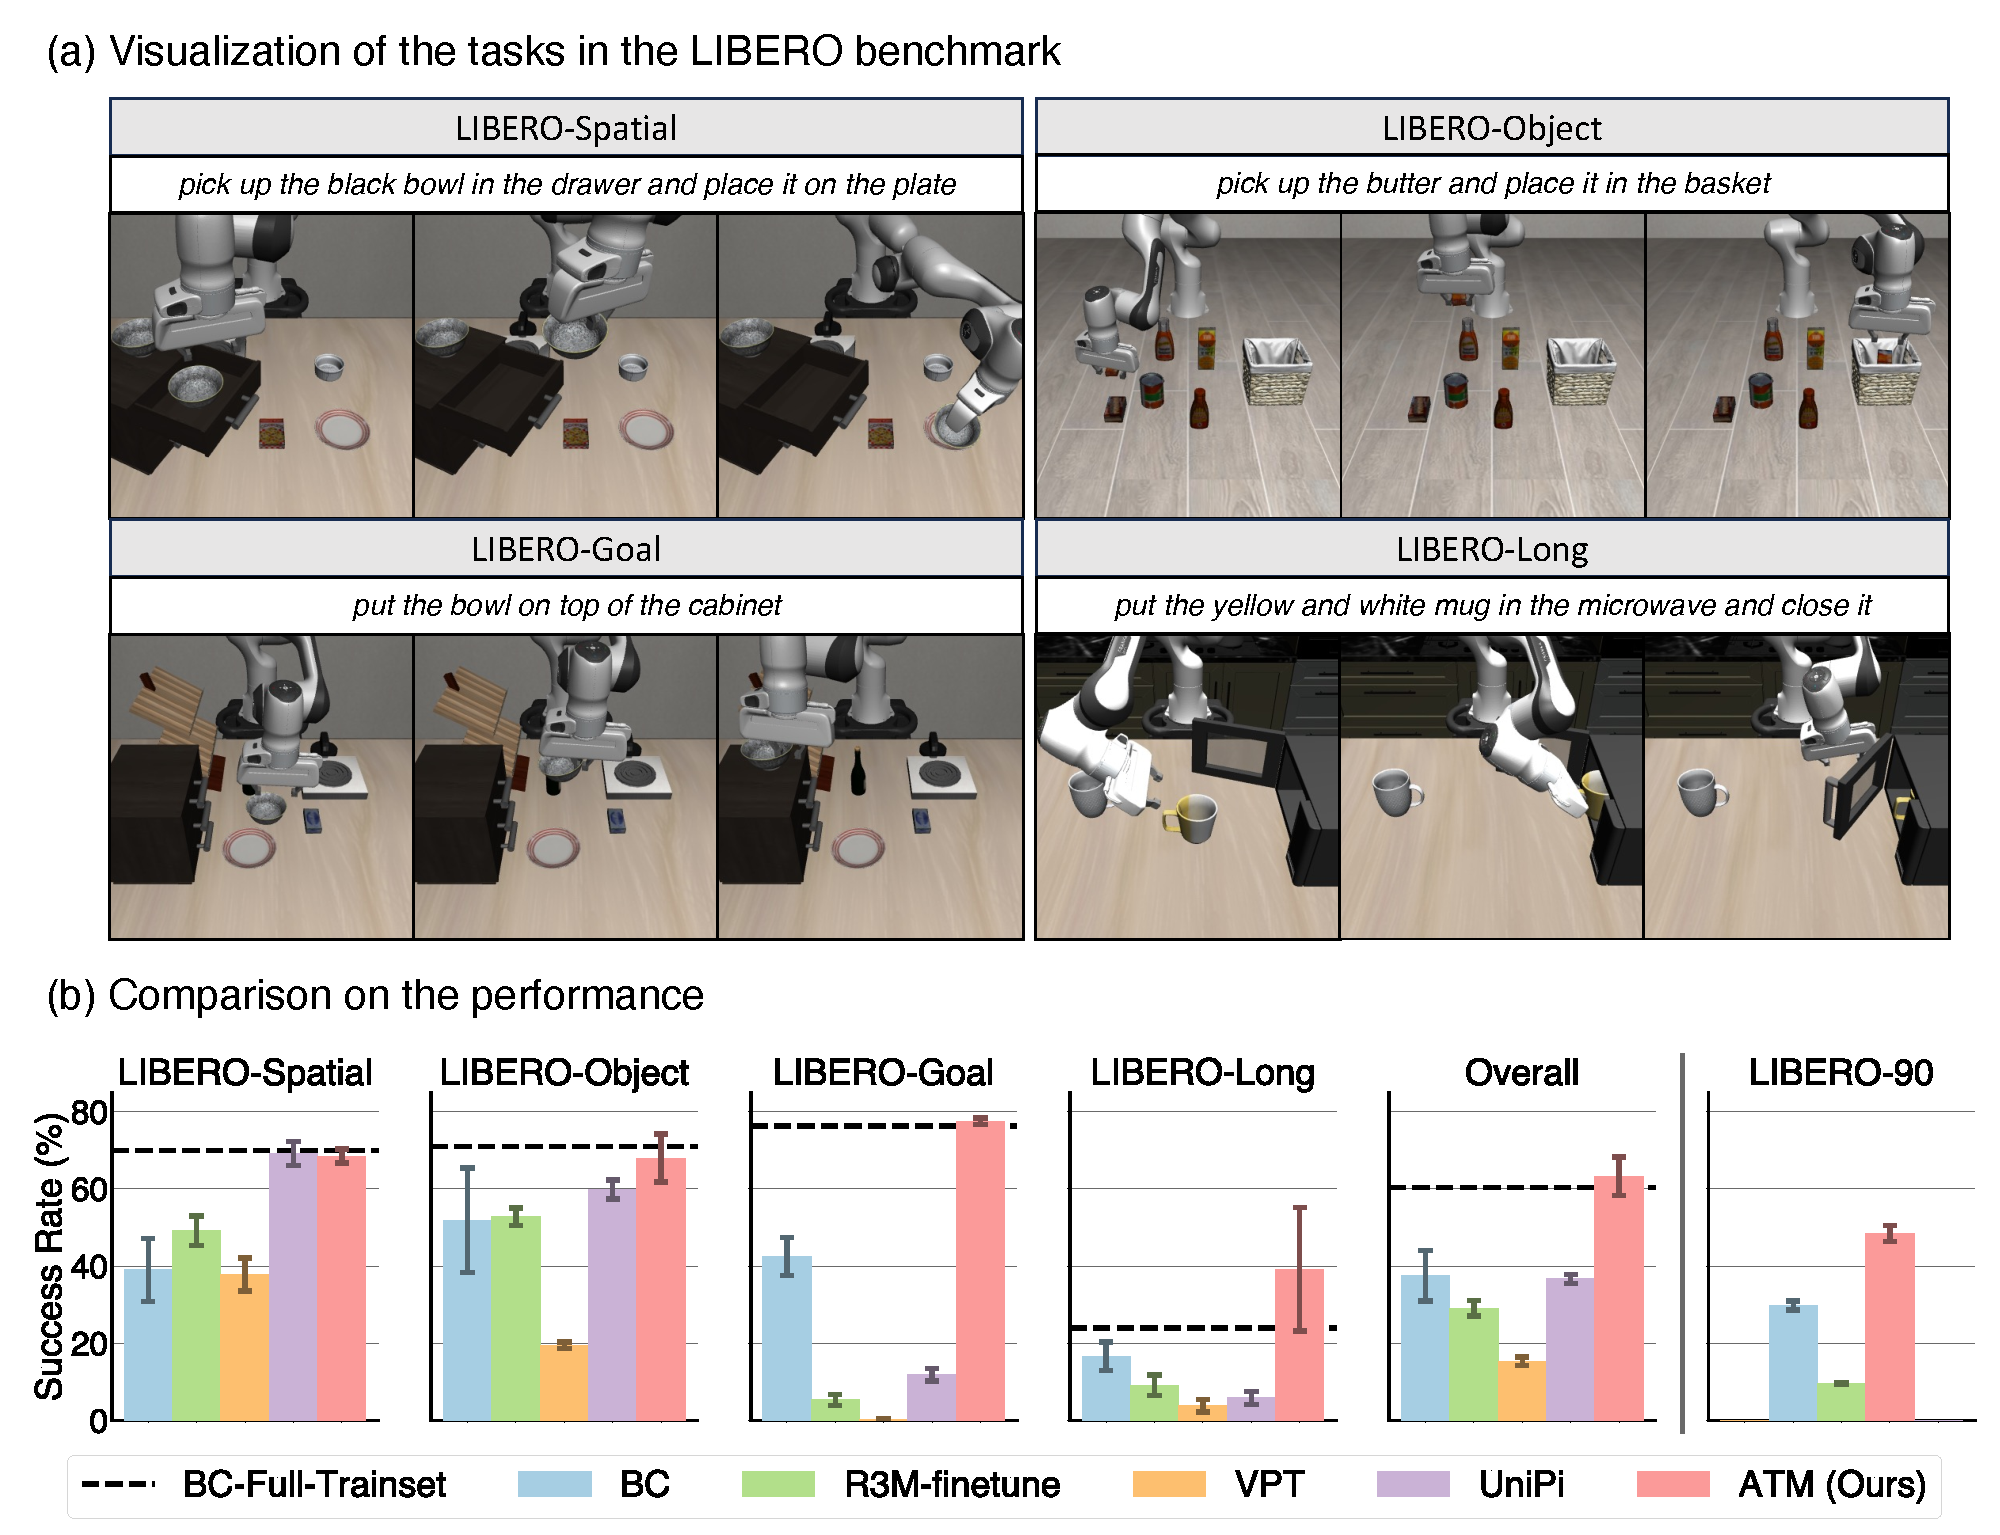
\includegraphics[width=\linewidth]{fig/sim_exp.pdf}
    \caption{我们在 LIBERO 基准指标中与语言条件操作任务的最先进的视频预训方法进行比较~\cite{liu2023libero}图: (a) 视觉化LibERO任务分为四个套件,重点关注空间推理,对象推理,任务理解和执行长视界任务的操纵策略的不同方面. (b) 对不同套件进行量化比较.我们还将基线与90项任务的任务套件 (即LibERO-90) 的快速计算进行比较.ATM在所有任务中优于基线,在 LIBERO-目标和 LIBERO-长方面优越.}
    \label{fig:sim_exp}
\end{figure*}

\begin{figure*}[ht]
    \centering
    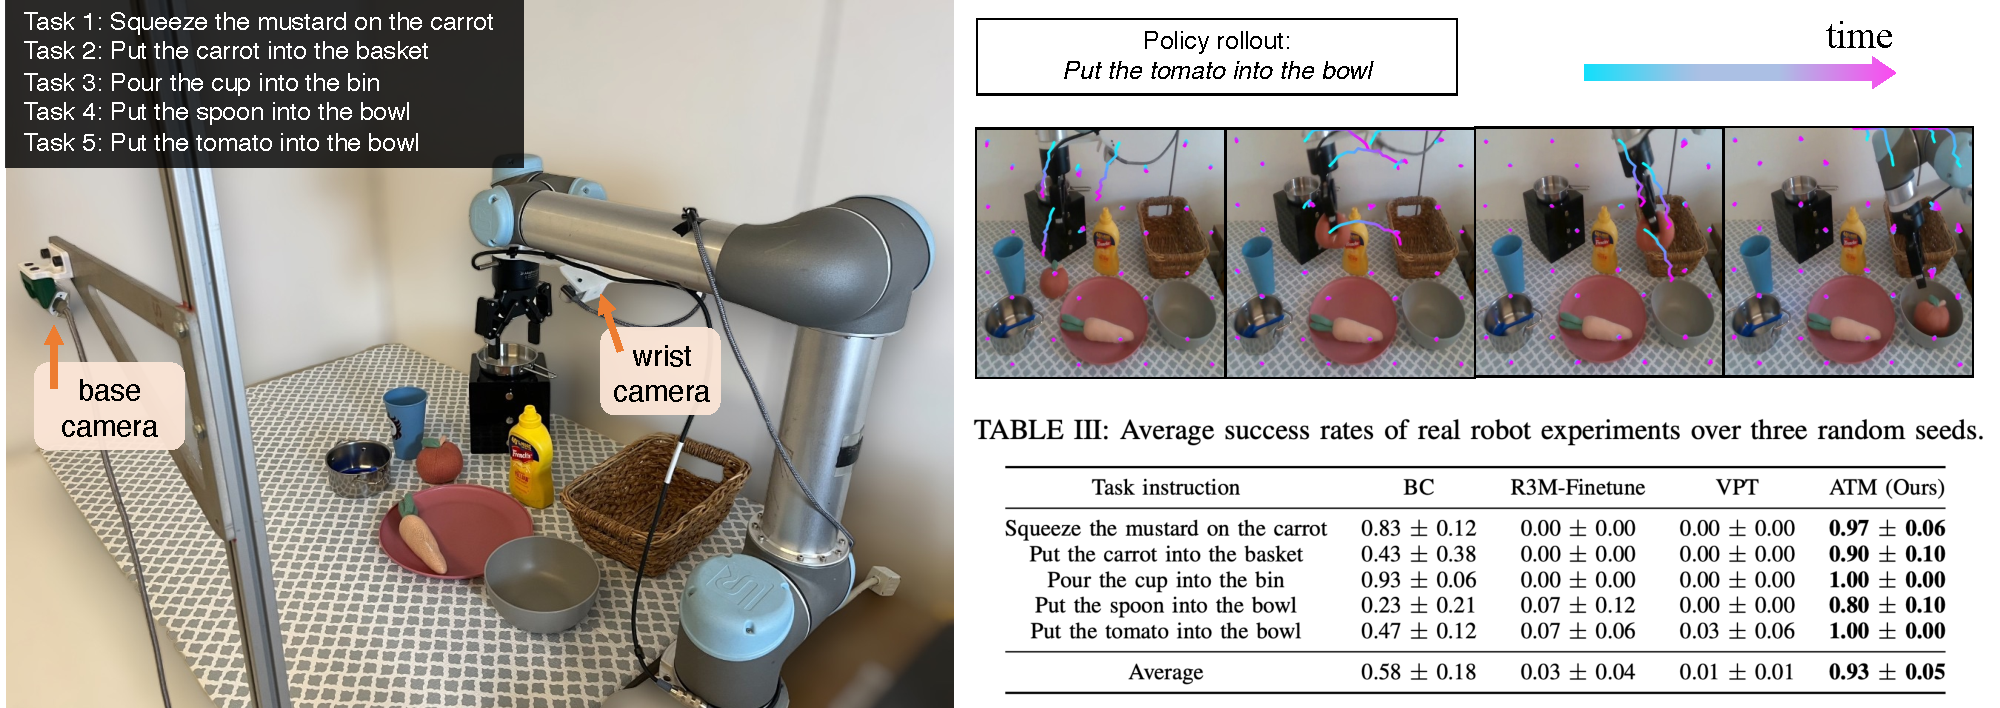
\includegraphics[width=\linewidth]{fig/real_exp.pdf}
    \caption{实际机器人实验在一个餐桌设置由五项任务组成.左图显示了我们的现实世界设置和任务.右图显示了预测粒子轨迹和策略执行的一个例子,紧随预测轨迹.从数量结果,我们可以看到ATM显示了显著的改善与最先进的视频预训基线平均.}
    \label{fig:real_exp}
\end{figure*}

\subsection{视频 预训练 模仿学习}~\label{sec:video_bc}
我们在 LIBERO 基准指标中对100多项语言条件操作任务进行了基线比较~\cite{liu2023libero}基准分为五个套件,LibERO-Space,LibERO-Object,LibERO-Goal,LibERO-Long和LibERO-90.每套件都有10个任务,除了LibERO-90包含90个任务.每个任务都包含专家人类示范.LibERO-Spatial包含具有相同的对象,但不同布局的任务;LibERO-Object具有相同的布局,但不同的对象的任务;LibERO-Goal具有相同的对象类别和空间布局,但不同的目标;LibERO-Long具有多种对象类别和布局,以及长视野任务目标;LibERO-90具有极其多种的对象类别,布局和任务目标.

我们将每个套件的基线单独进行比较. $10$ 动作标签的示范轨迹 $50$ 无动作视频示范轨迹,为每项任务, $500$ 展示数据集包含来自第三方摄像头和手腕摄像头的RGB图像,以及抓住器和关节状态作为观察.由于每个任务是由语言指令指定的,我们使用预训练的BERT网络来获得任务嵌入~\cite{devlin2019-bert}图像分辨率是 $128\times128$ 它们是指向向向向向向向向向向向向向向向向向向向向向向向向向向向向向向向向向向向向向向向向向向向向向向向向向向向向向向向向向向向向向向向向向向向向向向向向向向向向向向向向向向向向向向向向向向向向向向向向向向向向向向向向向向向向向向向向向向向向向向向向向向向向向向向向向向向向向向向向向向向向向向向向向向向向向向向向向向向向向向向向向向向向向向向向向向向向向向向向向向向向向向向向向向向向向向向向向向向向向向向向向向向向向向向向向向向向向向向向向向向向向向向向向向向向向向向向向向向向向向向向向向向向向向向向向向向向向向向 

我们将其与以下基线进行比较:
\begin{enumerate}
    \item BC表示尼拉行为克隆,它仅使用有限的动作标签专家示范,而不使用视频数据集训练策略.它使用与ATM相同的策略架构,除了粒子轨迹被掩盖为零,而它取代语言嵌入为任务规范.BC基线也可以被视为没有行动视频的策略学习的废除.培训BC策略的具体架构和损失可能有所不同.我们使用BC来表示默认使用MSE损失训练的变压器策略,并对比该部分末尾单独与传播策略.
    \item  子子~\cite{nair2023r3m} 采用对比性学习目标来表达学习,使视频和语言与对比性时间损失的组合相一致, $L_{1}$ 我们采用公开发布的Ego4D预训练重量,并对我们在域内视频数据集中的重量进行细节调整. $\mathcal{T}_o$通过视觉表现学习,我们还可以通过视觉表现来捕捉无动作视频的前例. 虽然这种方法通过表现学习捕获了无动作视频的前例,但视觉表现缺乏对决策至关重要的过渡动态的知识.
    \item 的~\cite{baker2022vpt} 首先从动作标记轨迹中训练一个反动动态模型 $\mathcal{T}_a$ 通过这些伪标签,一个策略随后训练行为克隆. 这种方法要求反动动态模型强大于广泛的输入观察分布,这可能很难从有限的示范中学习. 
    \item 单一~\cite{du2023unipi, Ko2023Learning,black2023zero} 在学习策略期间,UniPi训练一个反向动态模型,使用动作标签数据. 我们将我们的实现建立在 UniPi的实现基础上.~\citet{Ko2023Learning}虽然UniPi和ATM都利用以未来的子目标为条件的策略,但轨迹表示将运动与其他基于像素的信息分离开来,使策略学习更加容易.请参阅附件,我们将对UniPi的不同变化进行进一步全面的比较. 
\end{enumerate}

结果. 我们在图中介绍了主要结果~\ref{fig:sim_exp}我们看到,通过将视频数据和策略学习与点轨迹结构化表示联系起来,~视频预训的不同强基线显著超过了我们的方法, $63\%$ 与最高的成功率相比 $37\%$ 通过以前的方法, 标志着改善 $80\%$比较BC与ATM显示,从额外的视频中学习为策略学习提供了有用的信息.VPT的性能很差,因为我们经验观察到,VPT预测的伪动作标签通常显示出视频数据集中的大错误.UniPi更复杂,因为视频预测模型不基于物理,并且经常生成未来的框架,不实质上可行,例如机器人从图像中消失的情况.ATM在长视线任务和需要了解目标的任务上表现出了惊人的优势.我们将这种性能归因于ATM的公式,该系统利用明确的粒子轨迹作为子目标.每次步骤,ATM根据当前的观察预测未来的目标轨迹.与其他方法使用的静态自然语言指令相比,这些方法在整个剧集中不会改变,ATM的闭环未来轨迹提供了明确的指导,说明该策略需要做什么.

预测轨迹的好处也可以用于流传策略等最先进的策略类别~\cite{Chi2023diffusion}图所示~\ref{fig:diff-policy-results}在这里,ATM扩散策略将预测的未来轨道添加为策略类的额外条件,同时保持其他一切相同.我们看到ATM在所有套件中持续改善了扩散策略的性能,在 LIBERO基准上取得了最高分数.更多详情可以在附件中找到.

\begin{figure}[ht]
    \centering
    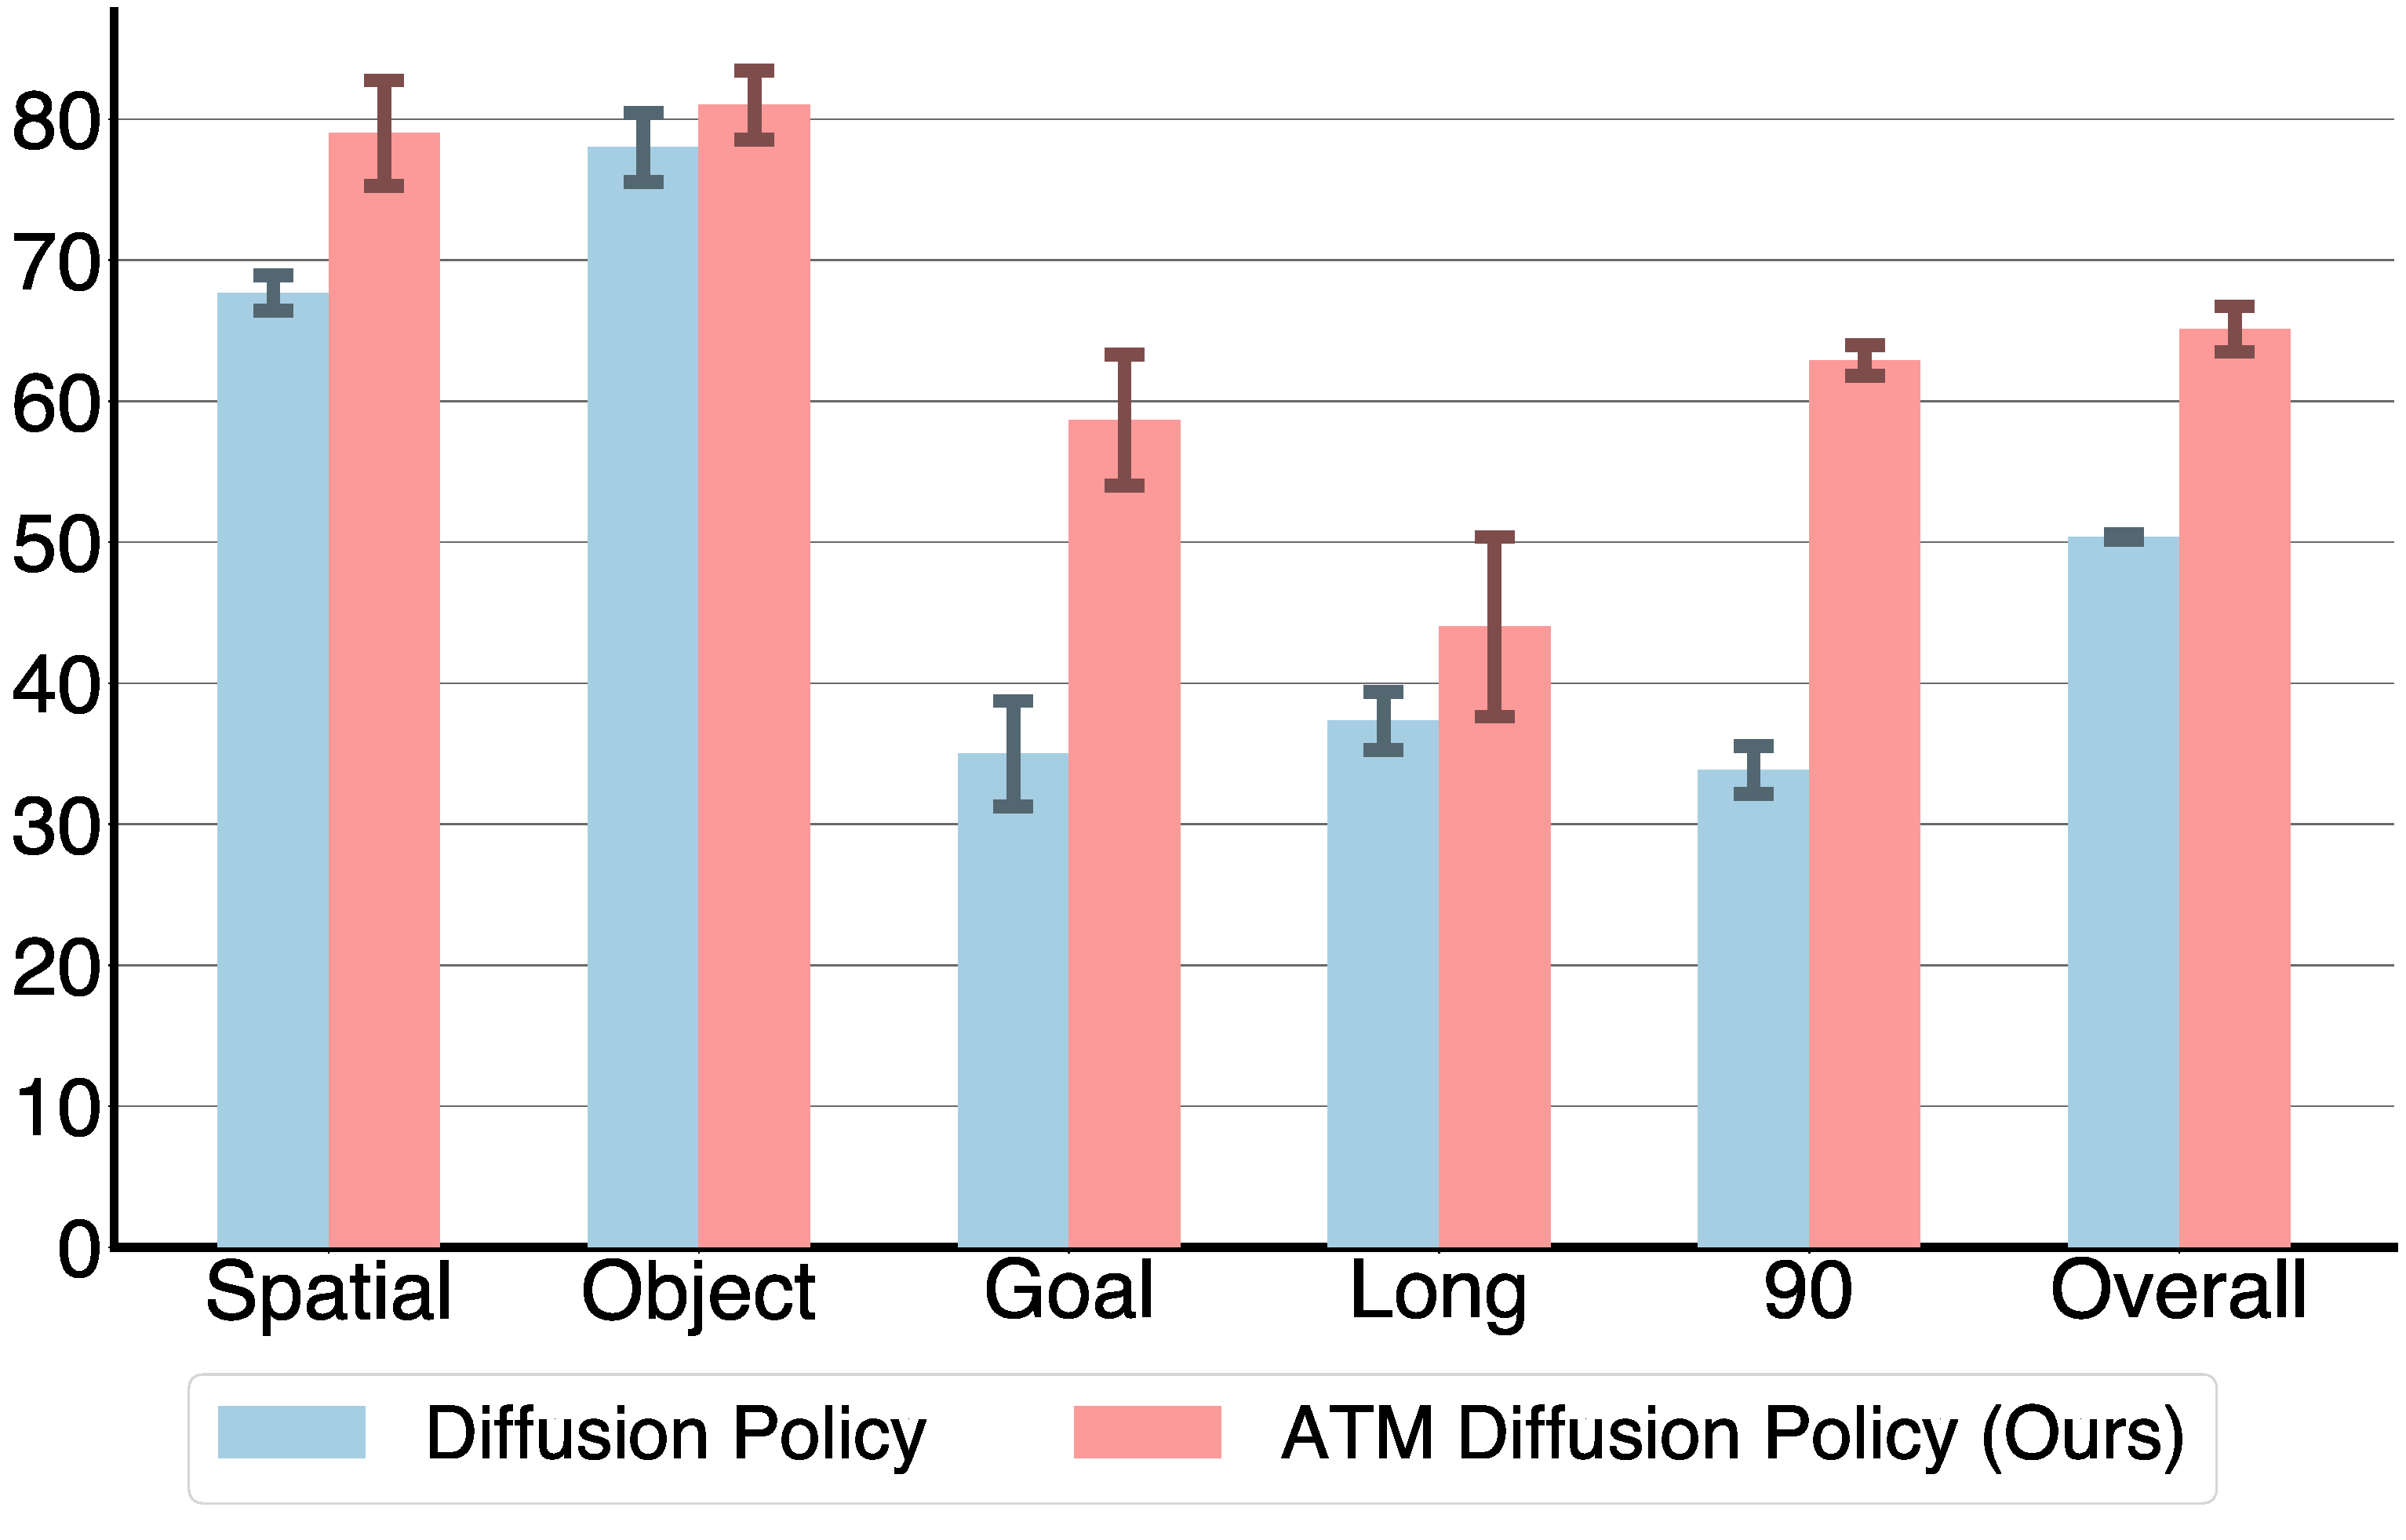
\includegraphics[width=\linewidth]{fig/libero-diffpolicy-success-rate.pdf}
    \caption{我们通过将预测未来轨迹添加为额外的条件,并显示了基准扩散策略的持续改善.}
    \label{fig:diff-policy-results}
\end{figure}

我们在现实世界中进行了语言调节的操纵实验,以进一步加强我们的声称.~\ref{fig:real_exp}通过采用GELLO远程操作系统收集的人类专家示范,我们学习了6DOF UR5机器人臂的策略~\cite{wu2023gello}行动空间是联合位置控制和抓住状态.观察包括两个RealSense摄像头的两个RGB图像.为了弥补部分观察,我们将最近的两个框架堆叠成代理的输入.我们不会将自觉状态输入到代理中,因为据报道,仿真策略往往过度适应它们并忽略视觉输入,导致在线推广性能更糟.~\cite{robomimic2021,lin2023spawnnet}我们收集了总数 $50$ 动作标签的轨迹 $250$ 通过简单地从收集的动作标签示范中删除行动的示范视频.~\ref{fig:real_exp}随着这些趋势,我们看到ATM在BC和其他视频预训基线上表现得更好.

\begin{figure*}[ht]
    \centering
    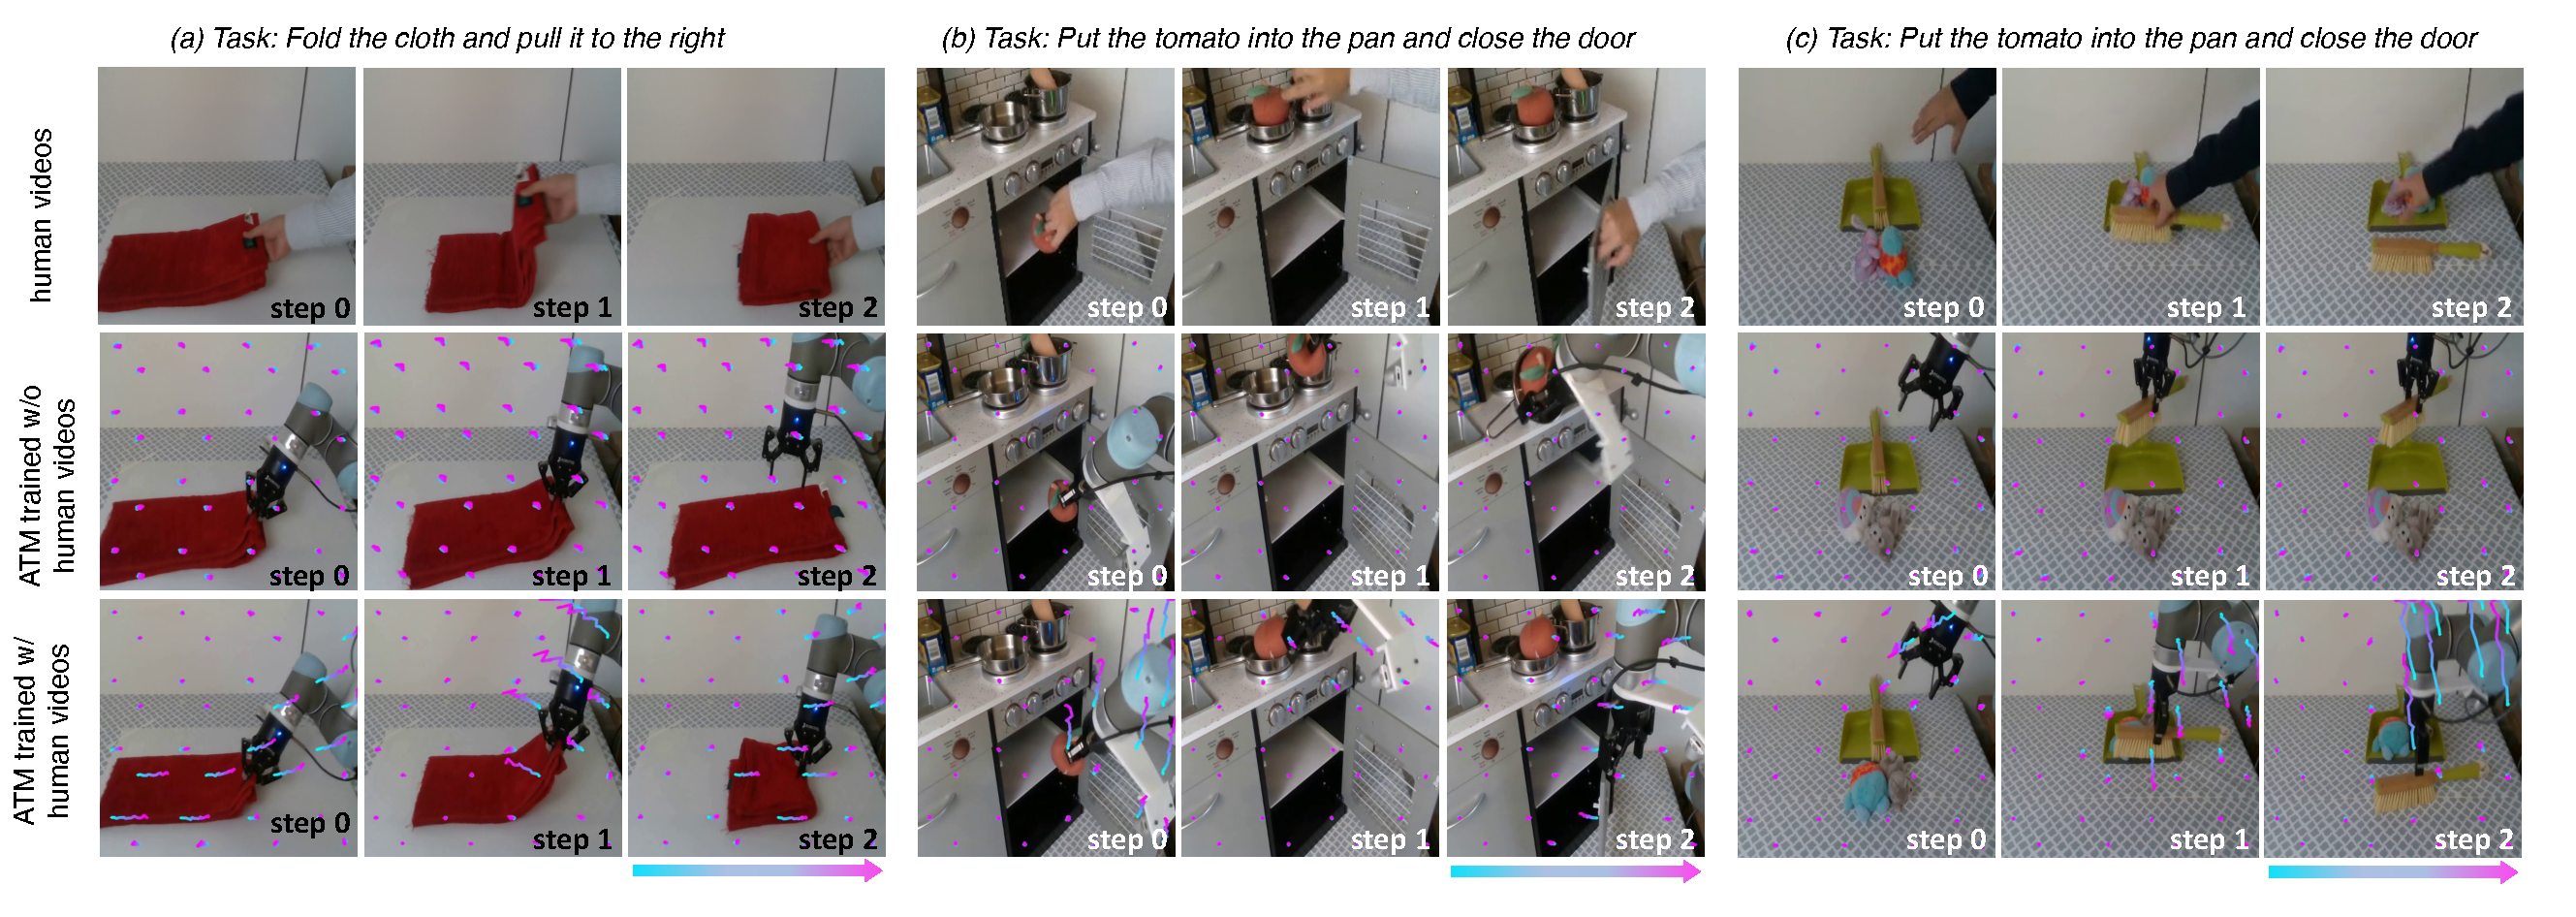
\includegraphics[width=\linewidth]{fig/human_video.pdf}
    \caption{通过人类视频学习机器人技能,完成三个任务.我们收集了100个人类直接执行任务的视频和10个遥控操作示范轨迹.从上到下面的每一行显示了人类视频的三个快照,无人视频训练的ATM和人类视频训练的ATM.比较来说,我们可以看到人类视频对于学习准确的轨迹预测至关重要,并使策略能够成功执行任务.}
    \label{fig:human_video}
\end{figure*}

\begin{figure*}[ht]
    \centering
    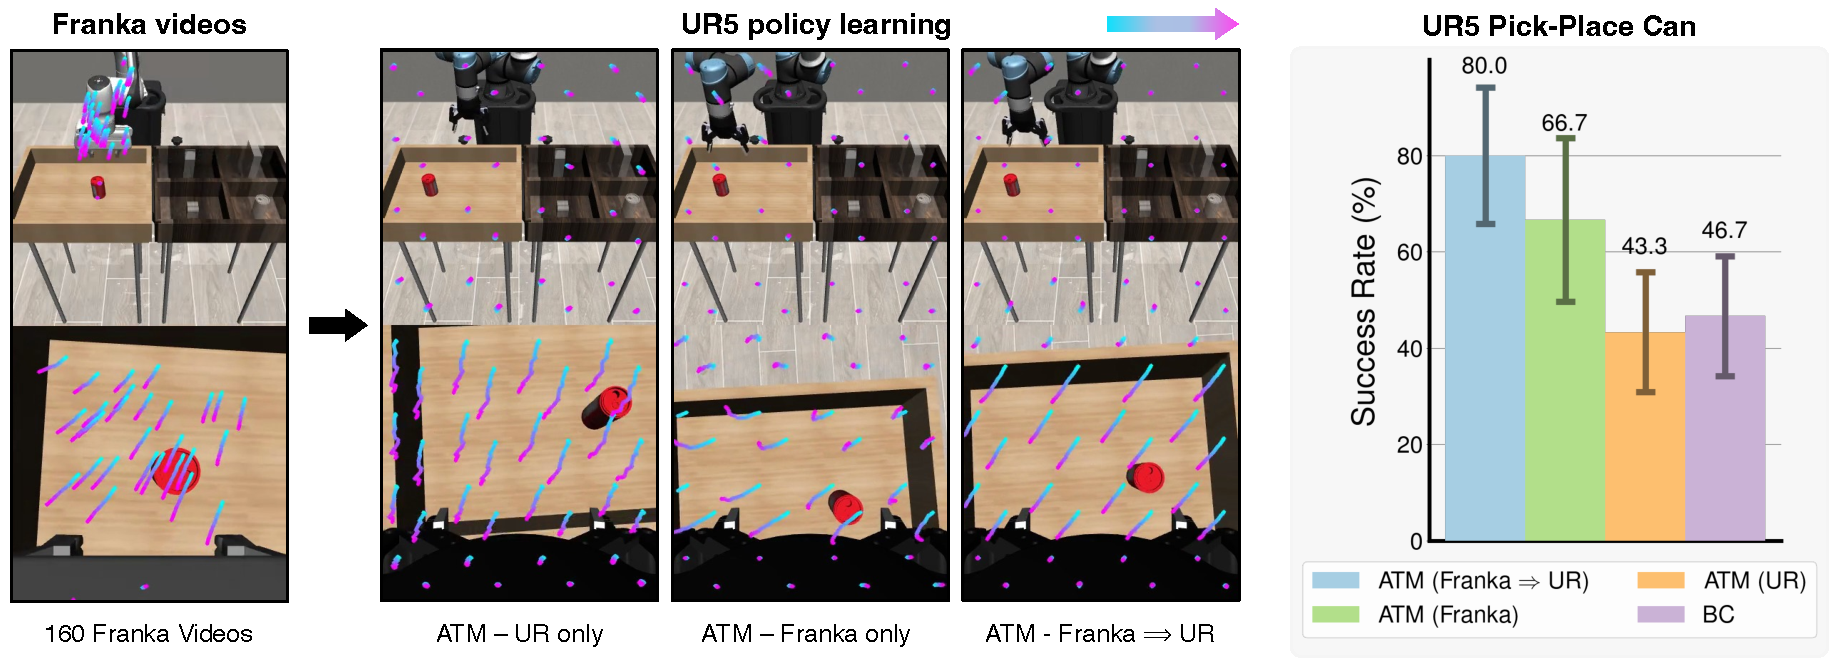
\includegraphics[width=\linewidth]{fig/rob-rob.pdf}
    \caption{在这里,我们收集了160个免动作视频的Franka手臂和10个标签的示范从一个 UR手臂,最终目标是学习一个 UR 策略.我们比较一个尼拉BC基线与ATM训练使用数据类型:仅使用10个 UR 视频,仅使用160个Franka 视频,并使用 Franka 和 UR 视频 (Franka 视频) $\Rightarrow$ 虽然这项轨迹模型仅使用了Franka视频,但它表现得比 BC没有Franka视频更好.}
    \label{fig:rob-rob}
\end{figure*}

\begin{table}[ht]
  \centering
  \caption{人与机器人实验的平均成功率.使用人类视频训练的ATM显著超过BC和仅使用10个机器人视频训练的ATM,证明了ATM的跨体体能力.}
  \begin{tabular}{@{}cccccc@{}}
    \toprule
     方法 & \specialcell{远程操作 \\ 演示} & \specialcell{人类 \\ 视频} & 折叠布 & 放茄 & 扫除玩具 \\
    \midrule
    美国 & \CheckmarkBold & \XSolidBrush & 0\% & 10\% & 30\% \\
    银行票 & \CheckmarkBold & \XSolidBrush & 0\% & 0\% & 13\% \\
    银行票 & \CheckmarkBold & \CheckmarkBold & 63\% & 63\% & 60\% \\
    \bottomrule
  \end{tabular}
  \label{tab:human-robot-result}
\end{table}

\subsection{人与机器人,机器人与机器人转移} \label{sec:human_video}
通过模拟低级任意点轨迹,ATM可以从人类或执行任务的不同机器人的跨体体视频中学习.这使得更容易使用更可扩展的数据来源.为了验证这一点,我们在图中介绍了从人类视频中学习的结果.~\ref{fig:human_video}根据表表表的数量结果,~\ref{tab:human-robot-result}机器人交叉转移的结果~\ref{fig:rob-rob}我们比较以下方法: (1) 仅使用动作标签的数据进行学习行为克隆策略 (2) 采用仅使用有限的动作标签的机器人数据训练的轨迹 Transformer,以及 (3) 采用无动作的人类和无动作标签的机器人数据训练的轨迹 Transformer.实验表明,在额外的跨具身式视频上训练轨道模型使轨道预测更加强大,准确,显著提高了策略学习.另一方面,由于动作标签的轨道数量很小,仅使用动作标签的轨道的BC基线失败.请参阅我们网站上的视频以更好的可视化. 


\subsection{废除分析} \label{sec:ablation}
我们在模拟中进行了一系列的缩实验,以证明我们的设计选择的影响.这些包括策略学习所需的动作标签轨迹数量,轨迹预测视界的影响,图像掩盖和后期轨迹融合.此外,我们还研究了 ATM的普遍性,用于不同的策略模型.

\begin{figure}[ht]
    \centering
    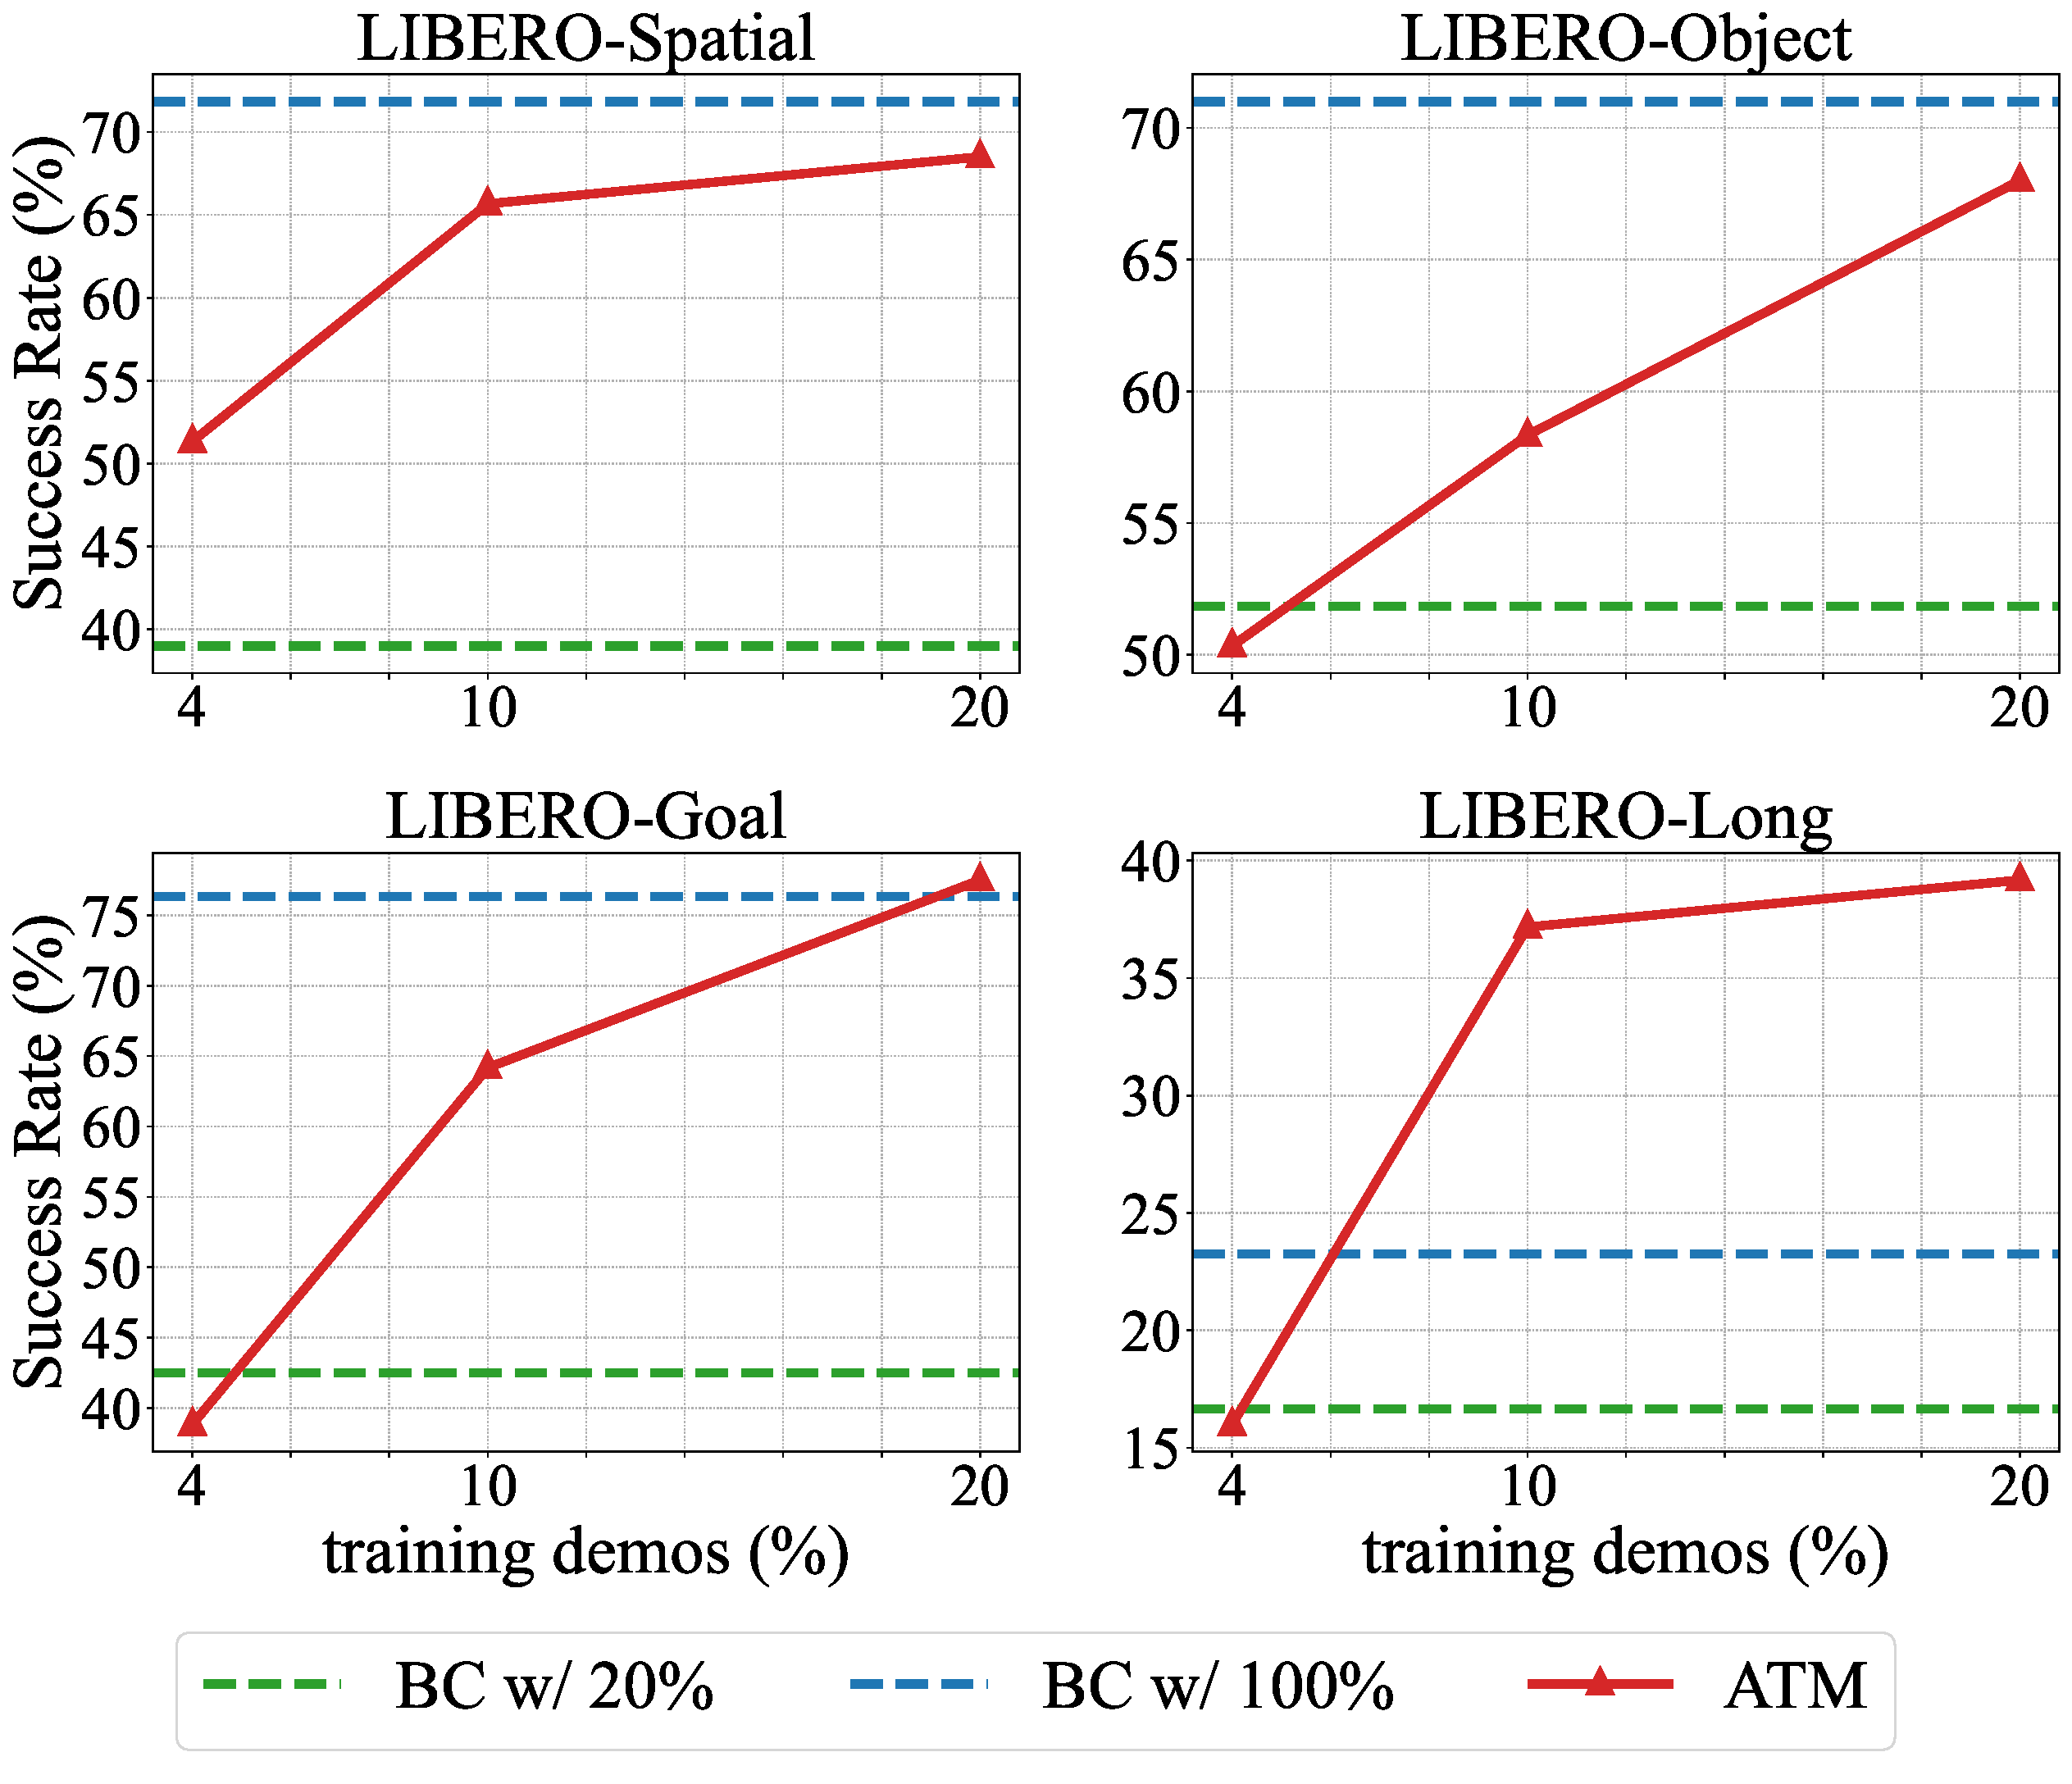
\includegraphics[width=\linewidth]{fig/libero-num-demos-with-bound.pdf}
    \caption{我们的策略成功率\%, 10\% 及20个\% 我们的策略只有4个\% 测试表现与BC基线相似,\% 在Libero-Spatial,Object,Goal,甚至更好的是在Libero-Spatial上.\% 我们的表现接近BC,所有的训练数据.}
    \label{fig:num-demos}
\end{figure}


通过使用预测的轨道长度的4,8,16,32和64步骤来训练我们的策略,我们研究了轨道长度对我们的策略输入的影响.如图所示~\ref{fig:libero-track-len}长度为16个轨道平均产生最佳性能.较小的轨道长度显著降低了性能,而长度为0的轨道长度将ATM降低到行为克隆基线,而没有预训练的任何好处.另一方面,较大的轨道长度也可能对性能产生负面影响,特别是在比利罗长度和利比罗目标等更具挑战性的任务上,因为长轨预测对于实现短视野子目标来说更有噪音,更不相关.确定子目标的最佳时间视野可能是未来研究的有趣途径.

\begin{figure}[ht]
    \centering
    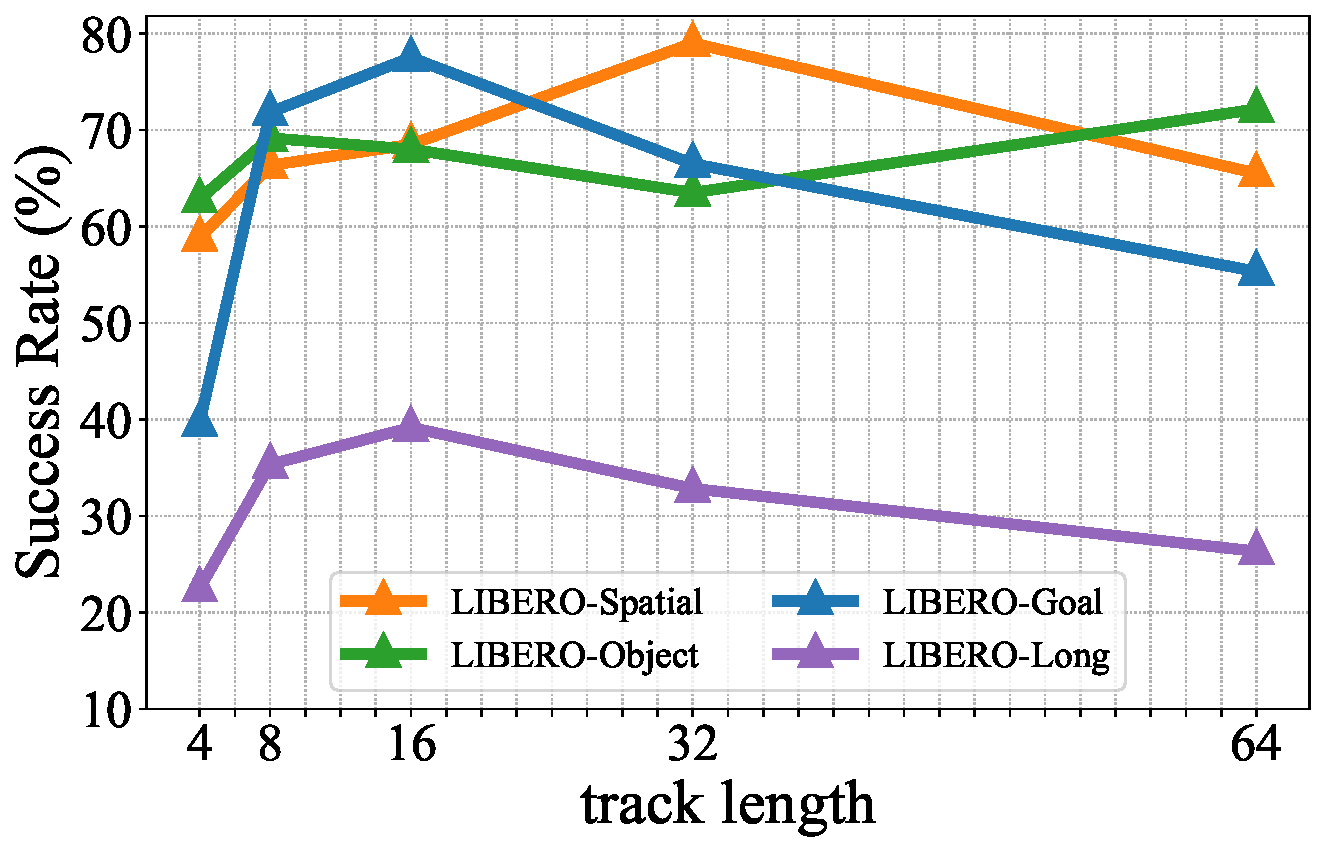
\includegraphics[width=0.9\linewidth]{fig/libero-track-length-longer.pdf}
    \caption{我们将使用不同的长度的预测轨迹来绘制所学到的策略的成功率.}
    \label{fig:libero-track-len}
\end{figure}

\begin{table*}[ht]
  \centering
  \caption{轨迹 Transformer的图像掩饰的除研究, ``面膜"表示在轨迹 Transformer训练中不掩盖图像补丁, ``图像掩盖"意味着我们随机掩盖50\% 我们可以看到,轨迹 Transformer中的面具图像建模提高了策略性能.}
  \begin{tabular}{@{}ccccc@{}}
    \toprule
    图像面具比例 & 空间 & 目标 & 目标 & 长时间 \\
    \midrule
    面膜图像 & $69.17\pm6.38$ & $65.00\pm3.89$ & $74.33\pm3.66$ & $30.83\pm11.43$ \\
    w/图像掩盖 (默认) & $68.50\pm1.78$ & $68.00\pm6.18$ & $77.83\pm0.82$ & $39.33\pm15.80$ \\
    \bottomrule
  \end{tabular}
  \label{tab:ablation-mask-ratio}
\end{table*}

\begin{table*}[ht]
  \centering
  \caption{分析了策略结构的废除研究. 我们在两个位置探索了策略中输入的轨道的影响:变压器输入 (早期融合) 和MLP头 (后期融合),如图所示~\ref{fig:track_policy}.}
  \begin{tabular}{@{}cccccc@{}}
    \toprule
    早期融合 & 后期融合 & 空间 & 目标 & 目标 & 长时间 \\
    \midrule
    \CheckmarkBold & \XSolidBrush & $44.67\pm1.84$ & $56.67\pm3.09$ & $5.33\pm0.24$ & $22.33\pm4.94$ \\
    \XSolidBrush & \CheckmarkBold & $65.50\pm3.89$ &  $60.00\pm1.47$ & $72.83\pm4.73$  & $42.76\pm14.62$ \\
    \midrule
    \CheckmarkBold & \CheckmarkBold & $68.50\pm1.78$ & $68.00\pm6.18$ & $77.83\pm0.82$ & $39.33\pm15.80$ \\
    \bottomrule
  \end{tabular}
  \label{tab:arch-ablation}
\end{table*}

轨道长度效果.我们的预训练轨迹 Transformer的轨道长度为16个,我们默认地使用每个轨道的16个点作为我们的策略输入. 在这个实验中,我们通过训练我们的策略,预测轨道缩小成4,8和16步骤,研究了我们的策略输入轨道长度的影响.~\ref{fig:libero-track-len} 证明长轨道总体导致更高的成功率,除了LIBERO-Object,其中轨道长度 $=8$ 长轨道为每个任务提供更详细和具体的子目标,这对于指导代理的运动和行动在后期阶段至关重要.相反,对于LibERO-Object,该项目强调精度操作,而不是理解任务目标,一个长度16的策略与长度8的模型相比略低的性能.我们假设长轨道可能会干扰由于噪音而反动动态的学习.这也支持我们使用自然轨道作为次动态条件和利用反动态的方法.


轨迹 Transformer中的图像掩饰效果.训练轨迹 Transformer时,我们随机掩盖图像中的补丁,并学习重建它们作为辅助任务.我们通过删除图像掩饰损失并将其与我们的标准配置进行比较,我们随机掩盖. $50\%$ 图像面具的表格~\ref{tab:ablation-mask-ratio}图像掩饰被遗漏时,图像掩饰的性能略有下降,这表明图像掩饰可以成为有用的辅助任务,除了LibERO-Space.我们假设辅助损失鼓励模型共同推理图像观测的不同区域.这种偏见可能对Libero-Space任务不至关重要,因为特定的空间位置已经完全指定在语言说明中 (例如,所有任务都有"在 [某些空间位置]上拿起黑碗"格式). 图像掩饰的功能在图像的不同区域中,可以被视为具有影响力的. 

早期和晚期融合在策略架构的影响.~\ref{fig:track_policy}预测的轨道在策略内变压器架构之前和之后都被输入到策略中,我们分别称之为早期融合和后期融合.~\ref{tab:arch-ablation}通过结,我们可以看到,取消迟结导致性能下降;在LIBERO-Goal上,只有早期结的表现类似于其他基线,而只有迟结的表现略低于我们的全方位方法.这表明预测的轨道的迟结作为有用的子目标,帮助策略更好地理解多任务学习环境中的任务.由于在更大的视频数据集上训练,因此子目标预测更强大.
\section{限制}
我们的方法仍然依赖于一组标签的行动示范轨迹,从而限制了学习的策略的通用化.未来的工作可以考虑使用增强学习学习学习轨迹遵循的策略,以便不需要额外的示范数据.我们的方法的另一个限制是,我们在本文中使用的视频数据集仅包含小域空白.从野生视频数据集中学习带来多模式分布,多种摄像头运动和次优势运动等额外的挑战.我们将这些扩展留给未来的工作. 


\section{结论}
在本文中,我们将视频预训练中介绍一个任意点轨迹建模框架,有效地从无动作视频数据集中学习行为和动态.经过预训练,通过学习轨迹引导的策略,我们证明了与以前的最先进方法相比的显著改善,并显示出从未经过分发的人类视频中有效的学习.我们表明,基于粒子的表示可解释,结构化,自然包含物体永久性等物理诱导偏见.我们希望我们的作品将打开更多令人兴奋的方向学习从结构化表示的视频中.


\section{认可}
这项工作由BAIR工业联盟和香港特别行政区政府的InnoHK通过香港物流机器人中心部分支持.这项工作也得到了中国人民共和国科学技术部的支持,即2030年创新大项目. ``关于新一代人工智能计划" (补贴号2021AAA0150000),以及国家关键R\&华为项目 (2022ZD0161700). 文在伯克利大学访问时完成了这项工作.



%% Use plainnat to work nicely with natbib. 
\bibliographystyle{鱼}
\bibliography{references}

\clearpage
\appendices
\section{其他实验结果}

\subsection{模拟实验}

报告 LIBERO基准指数成功率的数值~\ref{tab:libero-results}所有方法都使用20$\%$ 其他演示轨迹,除了神经.~\ref{sec:app:unipi} 详细了解UniPi和UniPi-Replan的比较.

为了展示轨道如何引导该策略,我们可视化 BC的空间变压器和我们的方法中的空间 CLS 代币和 RGB 代币之间的注意地图.~\ref{fig:policy-attention-map} 具体来说,它在各自的示例任务中照顾奶酪,碗和葡萄酒瓶,而BC通常被无关区分散,突出了轨道的优越能力,因为更好的任务提示.


\subsection{关于UniPi基线的讨论}\label{sec:app:unipi}

单一~\cite{du2023unipi} 建议培训一种语言条件的视频传播模式 $f_\theta$ 在视频预训期间. 在策略学习期间, $o_0$ 语言 $l$首先,UniPi生成了所有未来框架. $\Tilde{o}_1, \dots \Tilde{o}_{T-1} = f_\theta (o_0, l)$ 然后学习一个反动力学模型, $a_t = \pi(o_t, \Tilde{o}_{t+1})$尽管如此,训练一个扩散模型预测完整的视频可能是计算密集的,因此,我们的论文中的UniPi实现遵循了 \citet{Ko2023Learning}我们预测的 $N=7$ 未来框架作为策略的子目标,标志着 $\Tilde{o}_1, \dots \Tilde{o}_N$在训练中,我们均地抽样 $N$ 在学习策略期间,我们培训一个目标条件的策略 $\pi(a_t, \text{done} | o_t, \Tilde{o}_{i})$在哪里 $i\in {1, \dots N}$ 是图像的子目标, $t$ 策略还预测完成的标志,以确定该标志应该何时从当前的子目标中转移 $\Tilde{o}_i$ 进入下一个子目标 $\Tilde{o}_{i+1}$由于ATM在UniPi上优越,可归因于两个原因.一是,ATM使用更结构化的点轨迹子目标表示.二是,ATM执行闭环推理,每一步都提出一个新的子目标,而UniPi的视频传播过程太慢,不能在每一步都引用. 

\begin{table}[ht]
    \centering
    \caption{计算成本和推断时间为不同的方法在V100GPU上.ATM执行轨迹生成而不是预测高维框架,使其成为最计算效率和可行的闭环控制.UniPi在开始使用视频传播模型开放循环未来目标生成,要求更高的计算资源.UniPi-Replan使用较小的模型生成较少的框架,导致稍快的生成.然而,其使用在闭环控制仍然是计算上的禁忌.}
    \begin{tabular}{c c c c}
    \toprule
    \multirow{2}{*}{计算} & \multicolumn{2}{c}{密切环节} & 开放环节 \\
    % \cline{2-4}
     &  银行票 & 单一计划 & 单一\\
    \midrule
    按一代的TFLOPS        & 1.56 & 13.09 & 39.29 \\
    每一代的时间  & 0.015 & 4.51   & 8.14  \\
    \bottomrule
    \end{tabular}
    \label{tab:runtime}
\end{table}

为了培训UniPi策略,我们采用样本 $o_{i}$ 从未来的框架 $o_{t}$ 在哪里 $t \in [t, t+t_{max}]$我们选择了 $t_{max}$ 对于每个任务组 ($t_{max} = 16$ 对于 LIBERO-Object 和 LIBERO-Spatial, $t_{max} = 50$ 为了减轻学习完成的标志时的数据集失衡,我们采样了 $o_{i}$ 作为下一个框架 10\% 我们在两种行动中都进行了MSE回归. $a_t$ 现在就完成了.

为了分离ATM的两个优势与UniPi相比,我们还将视频预测模型训练来预测未来的固定时间步骤. $\Tilde{o}_{t+H}= f_\theta(o_t)$ 对于每一个 $H$ 策略执行的步骤, $H=8$由于这种变化更频繁地重新规划了子目标,我们将这种方法称为UniPi-Replan,类似于在~\cite{black2023zero}结果如表所示.~\ref{tab:libero-results}惊人的的是,我们发现这种变化比UniPi更糟糕.因此我们得出结论,一个结构化子目标表示可以比图像子目标更有效.原因是,在固定的未来时间步骤中预测图像目标可能是视频预测模型的困难目标,导致不一致的子目标.请参阅我们的网站上各种基线的故障视频.此外,这种方法需要大量计算.需要的计算的比较可以在表中显示~\ref{tab:runtime}由于计算成本,我们只评估UniPi-Replan在 LIBERO-Object和 LIBERO-Goal上,并报告了10次试验中的平均成功,




\begin{figure*}[ht]
    \centering
    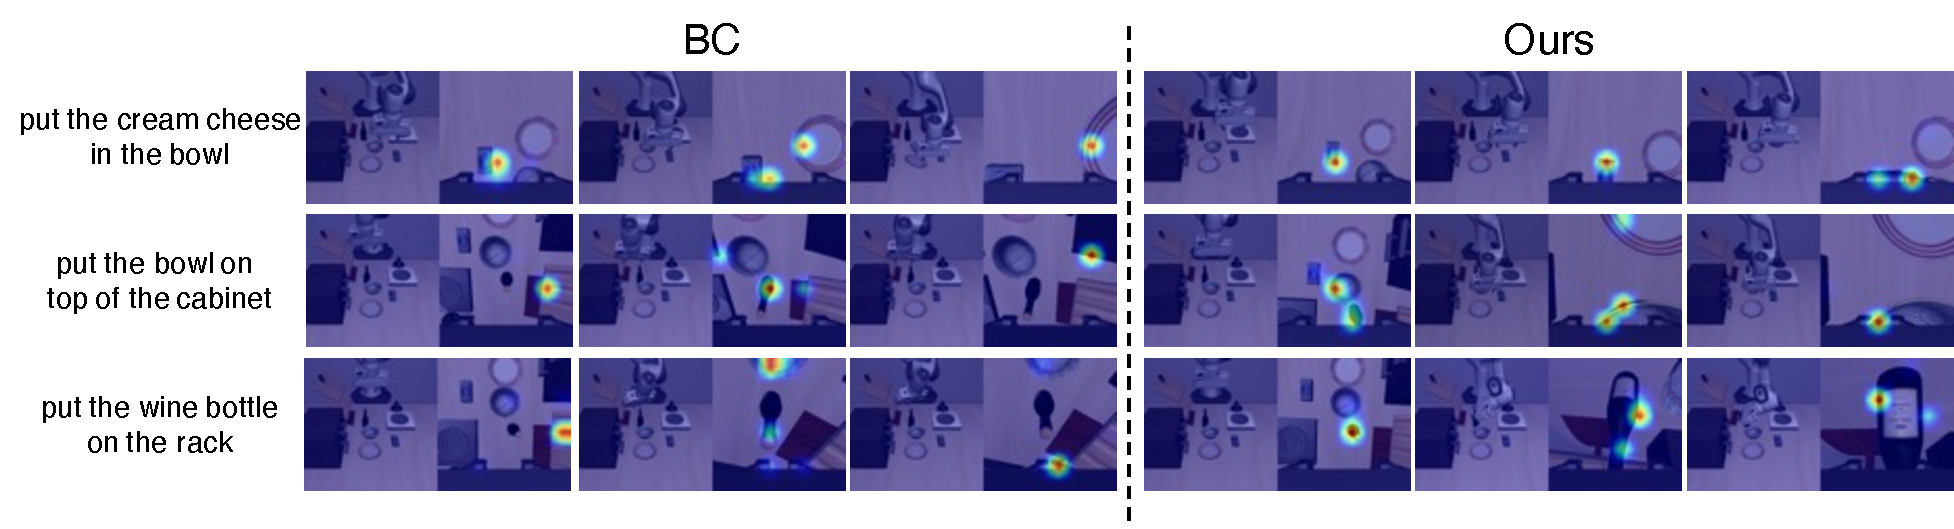
\includegraphics[width=0.95\linewidth]{fig/attention_map.pdf}
    \caption{空间变压器中的BC和我们的注意力地图.我们提取空间CLS标志和RGB标志之间的注意力权重,突出策略的关注特定空间区域在决策过程中.热地图显示了我们的策略的针对性关注任务相关领域,而BC倾向于关注无关背景.这突出了空间变压器中的输入轨道作为良好的任务提示,引导CLS标志进入适当领域.}
    \label{fig:policy-attention-map}
\end{figure*}

\begin{table*}[ht]
  \centering
  \caption{根据 LIBERO 基准,我们的方法的平均成功率比所有基线都不变.由于计算成本,UniPi-Replan仅为单个种子进行评估.}
  \begin{tabular}{@{}ccccccc@{}}
    \toprule
    方法 & 空间自由 & 自由对象 & 自由目标 & 自由长期 & 利贝罗-90 \\
    \midrule
    预测时间: & $71.83\pm3.70$ & $71.00\pm7.97$ & $76.33\pm1.31$ & $24.17\pm2.59$ & - \\
    \midrule
    美国 & $39.00\pm8.20$ & $51.83\pm13.54$ & $42.50\pm4.95$ & $16.67\pm3.66$ & $29.78\pm1.14$ \\
    子子~\cite{nair2023r3m} & $49.17\pm3.79$ & $52.83\pm2.25$ & $5.33\pm1.43$ & $9.17\pm2.66$ & $9.59\pm0.27$ \\
    的~\cite{baker2022vpt} & $37.83\pm4.29$ & $19.50\pm0.82$ & $3.33\pm2.36$ & $3.83\pm1.65$ & - \\
    单一~\cite{du2023unipi,Ko2023Learning} & $\bf 69.17 \pm 3.75$ & $59.83 \pm 3.01$ & $11.83 \pm 2.02$ & $5.83 \pm 2.08$ & - \\
    单一型反弹器~\cite{black2023zero} & - & 31.00 & 3.00 & - & - \\
    银行卡 (我们的) & $68.50\pm1.78$ & $\bf 68.00\pm6.18$ & $\bf 77.83\pm0.82$ & $\bf 39.33\pm15.80$ & $\bf 48.41\pm2.09$ \\
    \bottomrule
  \end{tabular}
  \label{tab:libero-results}
\end{table*}
 

\begin{figure}[ht]
  \centering
  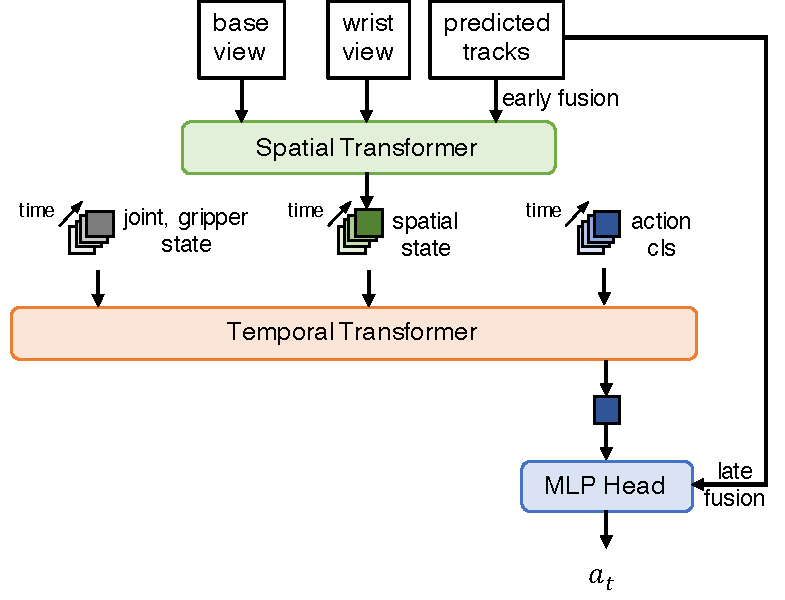
\includegraphics[width=0.9\linewidth]{fig/track_policy_app_simpler.pdf}
  \caption{为了总结空间信息,我们在一个由所有视图的跟踪和图像补丁和CLS标签组成的序列上进行自我注意.为了整合信息,我们在空间CLS标记,自觉感知和每步骤的行动CLS标记之间进行随机自我注意.为了退回行动,我们将每个步骤的行动CLS标记和建议的轨迹连接在一起. }
  \label{fig:arch-appendix}
\end{figure}

\begin{figure}[ht]
  \centering
  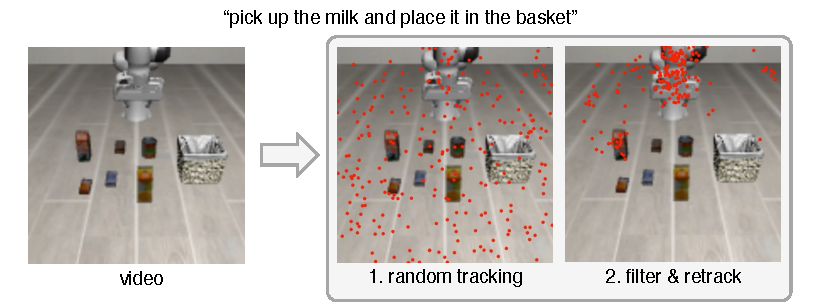
\includegraphics[width=\linewidth]{fig/filtering.pdf}
  \caption{视频 (左) 显示,我们采用现有TAP模型 (中部) 查询1000个随机抽样点,每个颜色点都代表了轨道的起点位置.然后我们通过视频中位置移动的选,重新样本这些点 (右).我们可以看到提取的轨道集中在信息物体,如机器人的抓住器和操纵目标.}
  \label{fig:filtering}
\end{figure}


\subsection{应用ATM到传播策略}
除了从原本的 LIBERO 文件中采用的变压器策略外,~\cite{liu2023libero}我们的ATM也可以与最先进的传播策略集成~\cite{Chi2023diffusion}具体来说,我们通过使用预测轨道作为输入条件实施了ATM传播策略.\% 根据图表的实验,~\ref{fig:sim_exp}.

图表所示~\ref{tab:diff-policy}尽管培训数据有限,但标准的LIBERO基准策略取得了令人印象深刻的成果,证实了其作为最先进的模仿策略的地位.


\begin{table*}[ht]
  \centering
  \caption{通过我们的方法可以进一步改善这种策略,这表明我们的任意点轨迹建模框架是任何策略模型应用的重要基石.}
  \begin{tabular}{@{}cccccc@{}}
    \toprule
    方法 & 空间自由 & 自由对象 & 自由目标 & 自由长期 & 利贝罗-90 \\
    \midrule
    传播策略 & $67.67\pm1.25$ & $78.00\pm2.45$ & $35.00\pm3.74$ & $37.33\pm2.05$  & $33.85\pm1.71$ \\
    银行卡扩散策略 & $79.00\pm3.74$ & $81.00\pm2.45$ & $58.67\pm4.64$ & $44.00\pm6.38$ & $62.89\pm1.10$ \\
    \bottomrule
  \end{tabular}
  \label{tab:diff-policy}
\end{table*}


\subsection{人与机器人传输详情}
为了展示ATM利用无限领域视频的潜力,我们在三个不同的设置中设计了人到机器人传输任务: 1) 可变形的对象:折叠布料并将其拉到右边, 2) 长视野:将番茄放进子里,关闭柜门, 3) 使用工具:使用扫扫玩具进入尘器,将其放进尘器前面.我们收集了10个机器人传输轨迹 (动作标签) 和100个人类操纵视频 (无动作比较).我们使用了三个方法: 1) 只有10个动作标签的机器人演示, 2) ATM,训练轨迹 Transformer,只有10个机器人演示, 3) ATM,训练一个轨迹 Transformer,使用无动作人类和无动作标签的机器人数据.~\ref{tab:human-robot-result}.

人到机器人视觉化. 人到机器人技能转移的详细视频视觉化如图~\ref{fig:human_video_supp}由于训练样本有限,仅使用10个机器人视频训练的轨迹 Transformer无法预测未来的点轨迹,导致成功率低.相反,使用人类视频训练的轨道模型在每个框架中生成高质量的轨迹,引导代理完成任务,仅使用10个动作标签的轨迹.这表明我们的任何点轨道建模能够将前进的运动从跨体体视频转移到机器人技能,这显著提高了策略学习.

另外,我们可以在图中看到训练有素的轨道变换器的注意力地图,~\ref{fig:tt-attention-map}轨迹 Transformer训练用人视频 (下行) 显示了精确的注意力热图,主要集中在对象和机器人臂上.相反,训练没有人视频的模型的注意力图 (中行) 显著分散,经常不准确地集中在背景区域. 这一比较突出了我们ATM在利用人类视频的先进知识的有效性,从而促进了成功的跨体体模仿学习.


\begin{table*}[ht]
\begin{minipage}[c]{0.48\textwidth}
\makeatletter\def\@型{桌子}
\centering
\caption{轨迹 Transformer训练的超参数.}
\begin{tabular}{@{}cc@{}}
    \toprule
    超参数 & 轨迹 Transformer \\
    \midrule
    时代 & 100  \\
    批量大小 &  1024  \\
    优化器 & 亚当W  \\
    学习率 & 1e-4  \\
    体重衰减 & 1e-4 \\
    时间表 & 子  \\\
    让你变暖 & 5 \\
    片类 & 10 \\
    点采样 & 变量过 \\
    积分数 & 32 \\
    轨道长度 & 16 \\
    轨道贴片大小 & 4 \\
    图像面具比例 & 0.5 \\
    增长 & 颜色,随机转换 \\
    \bottomrule
\end{tabular}
\label{tab:tt-hyperparameter}
\end{minipage}
\begin{minipage}[c]{0.48\textwidth}
\makeatletter\def\@型{桌子}
\centering
  \caption{策略培训的超级参数.}
  \begin{tabular}{@{}cc@{}}
    \toprule
    超参数 & 策略  \\
    \midrule
    时代 & 100  \\
    批量大小 &  512  \\
    优化器 &  亚当W  \\
    学习率 & 5e-4  \\
    体重衰减 & 1e-4 \\
    时间表 & 子  \\
    让你变暖 & 0 \\
    片类 & 100 \\
    点采样 & 网格 \\
    积分数 & 32 \\
    轨道长度 & 16 \\
    架 & 10 \\
    增长 & 颜色,随机转换 \\
    \bottomrule
  \end{tabular}
  \label{tab:policy-hyperparameter}
\end{minipage}
\end{table*}


\begin{figure*}
    \centering
    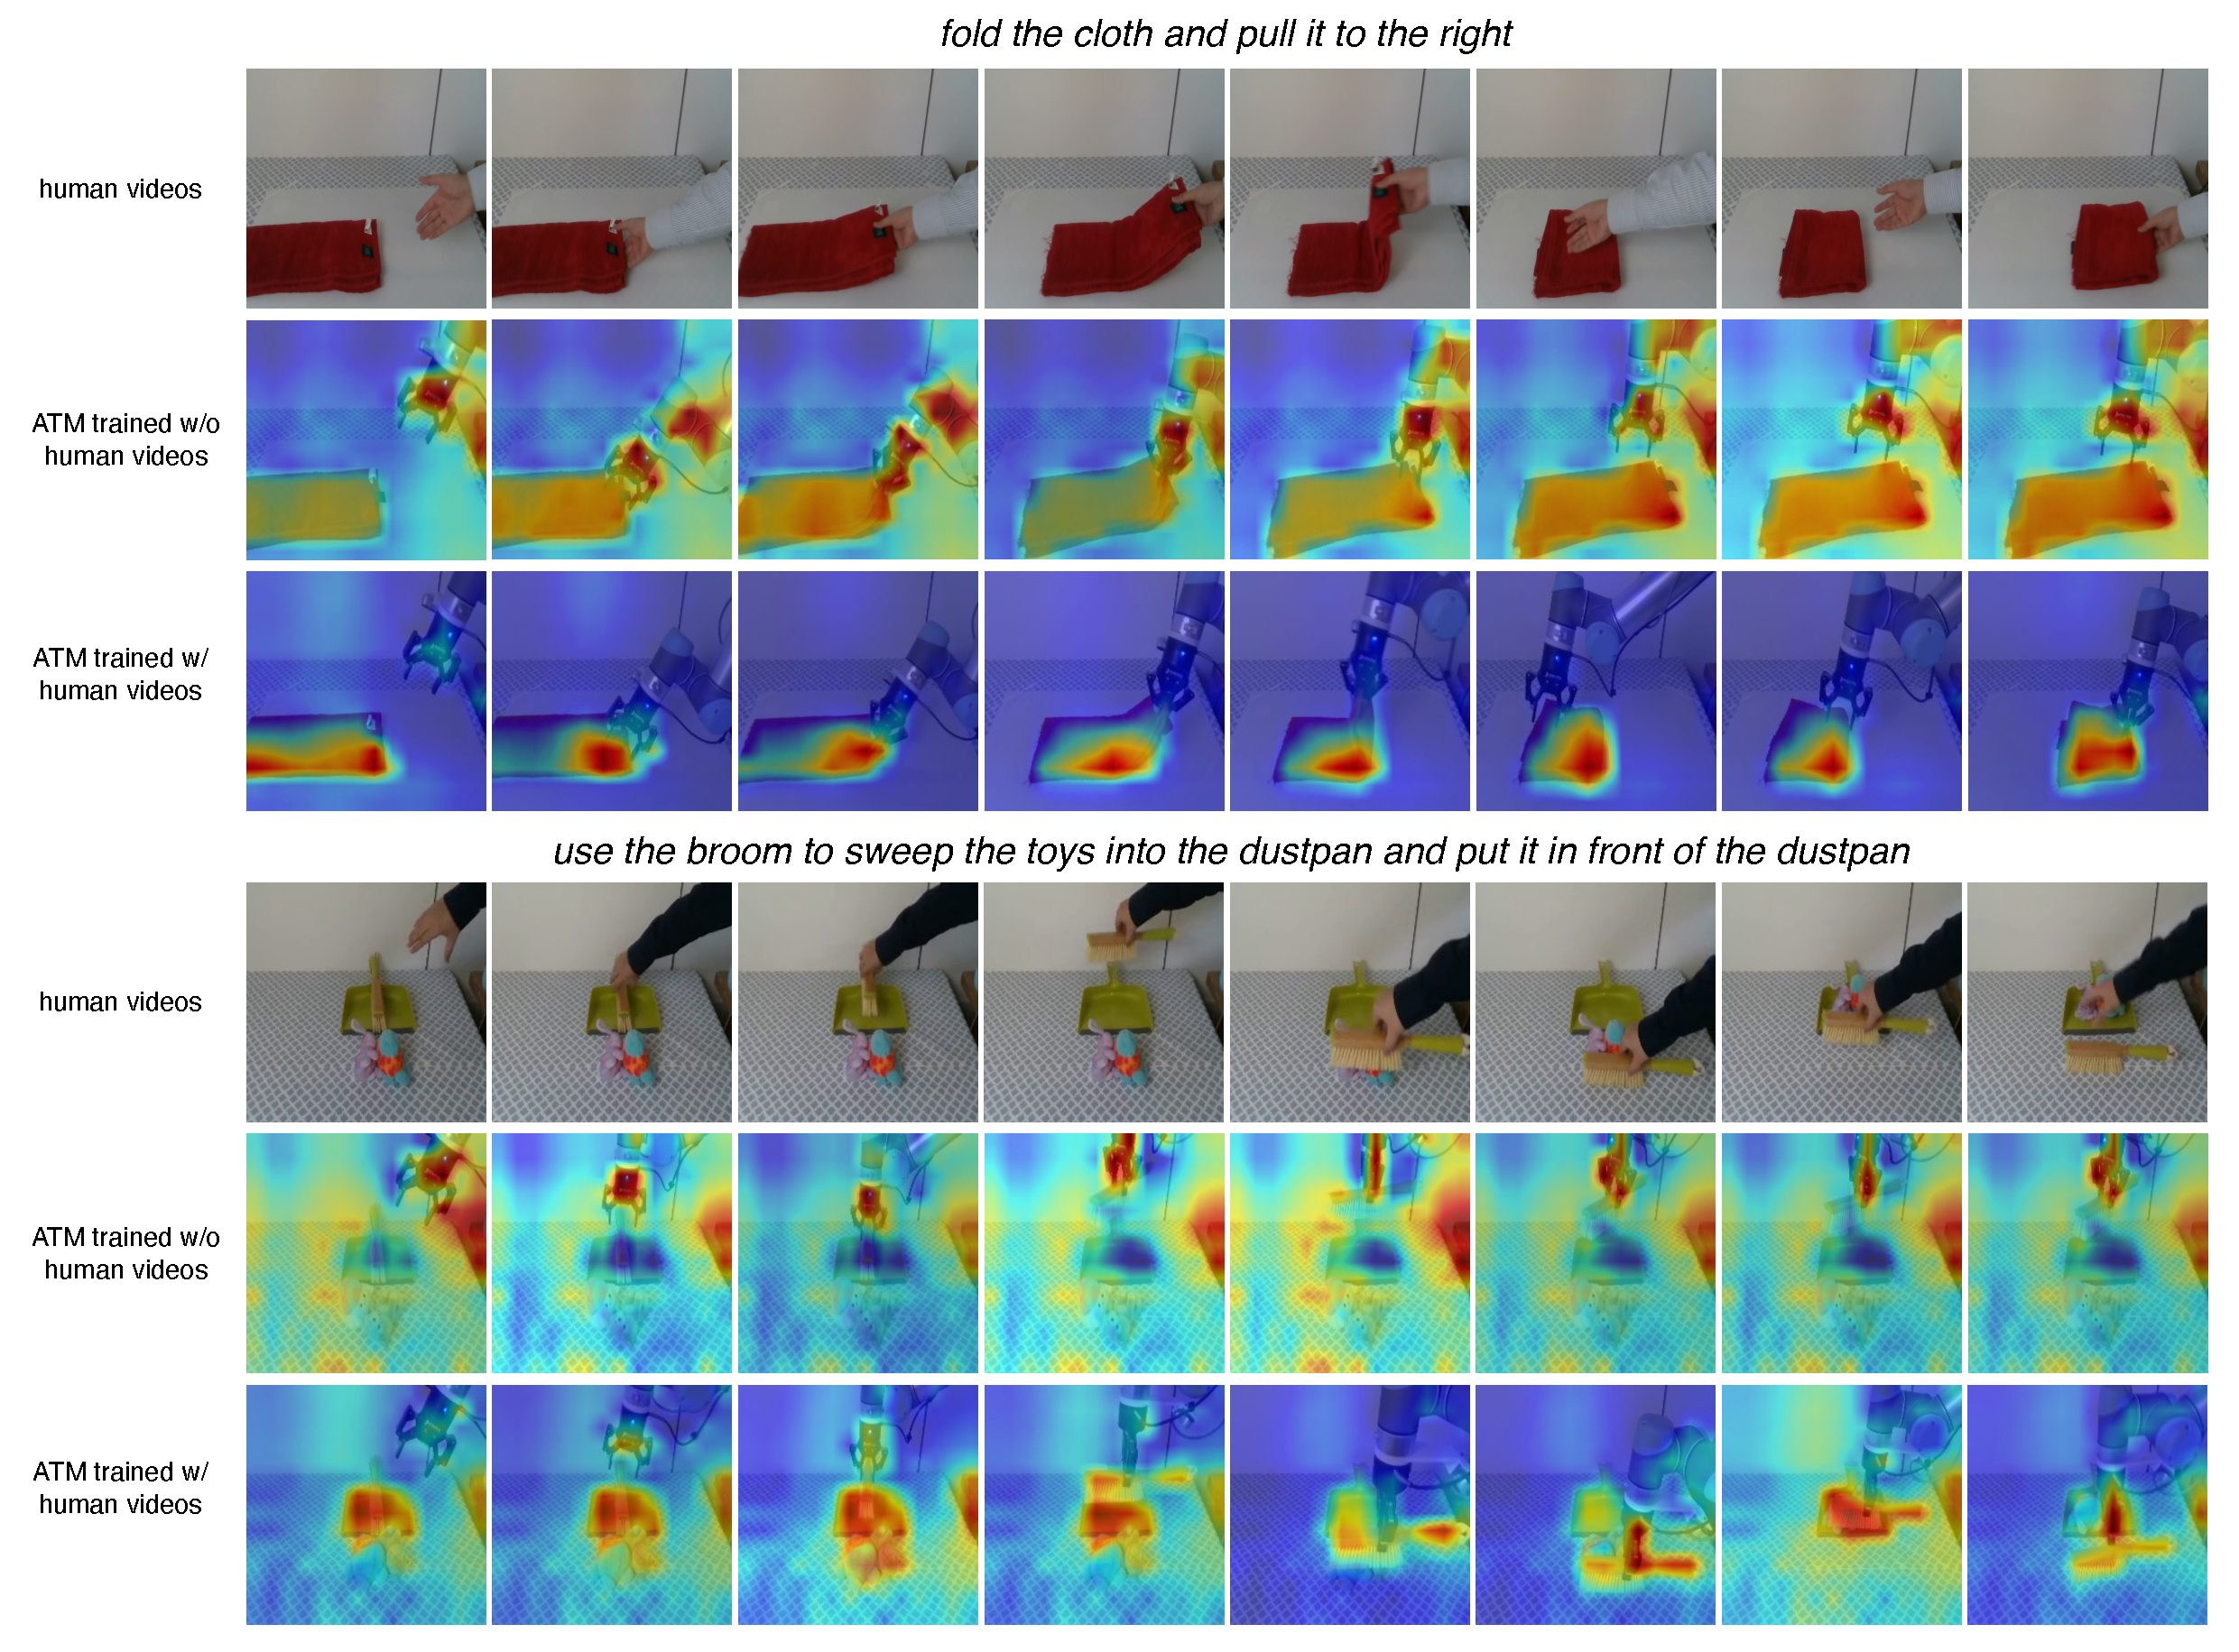
\includegraphics[width=0.95\linewidth]{fig/human_video_attn_rebuttal.pdf}
    \caption{视频包括大规模的人类视频,导致更清晰的注意力地图,专注于对象和机器人臂,而没有人视频的训练将关注不对的区域,如背景墙.}
    \label{fig:tt-attention-map}
\end{figure*}

\begin{figure*}[ht]
    \centering
    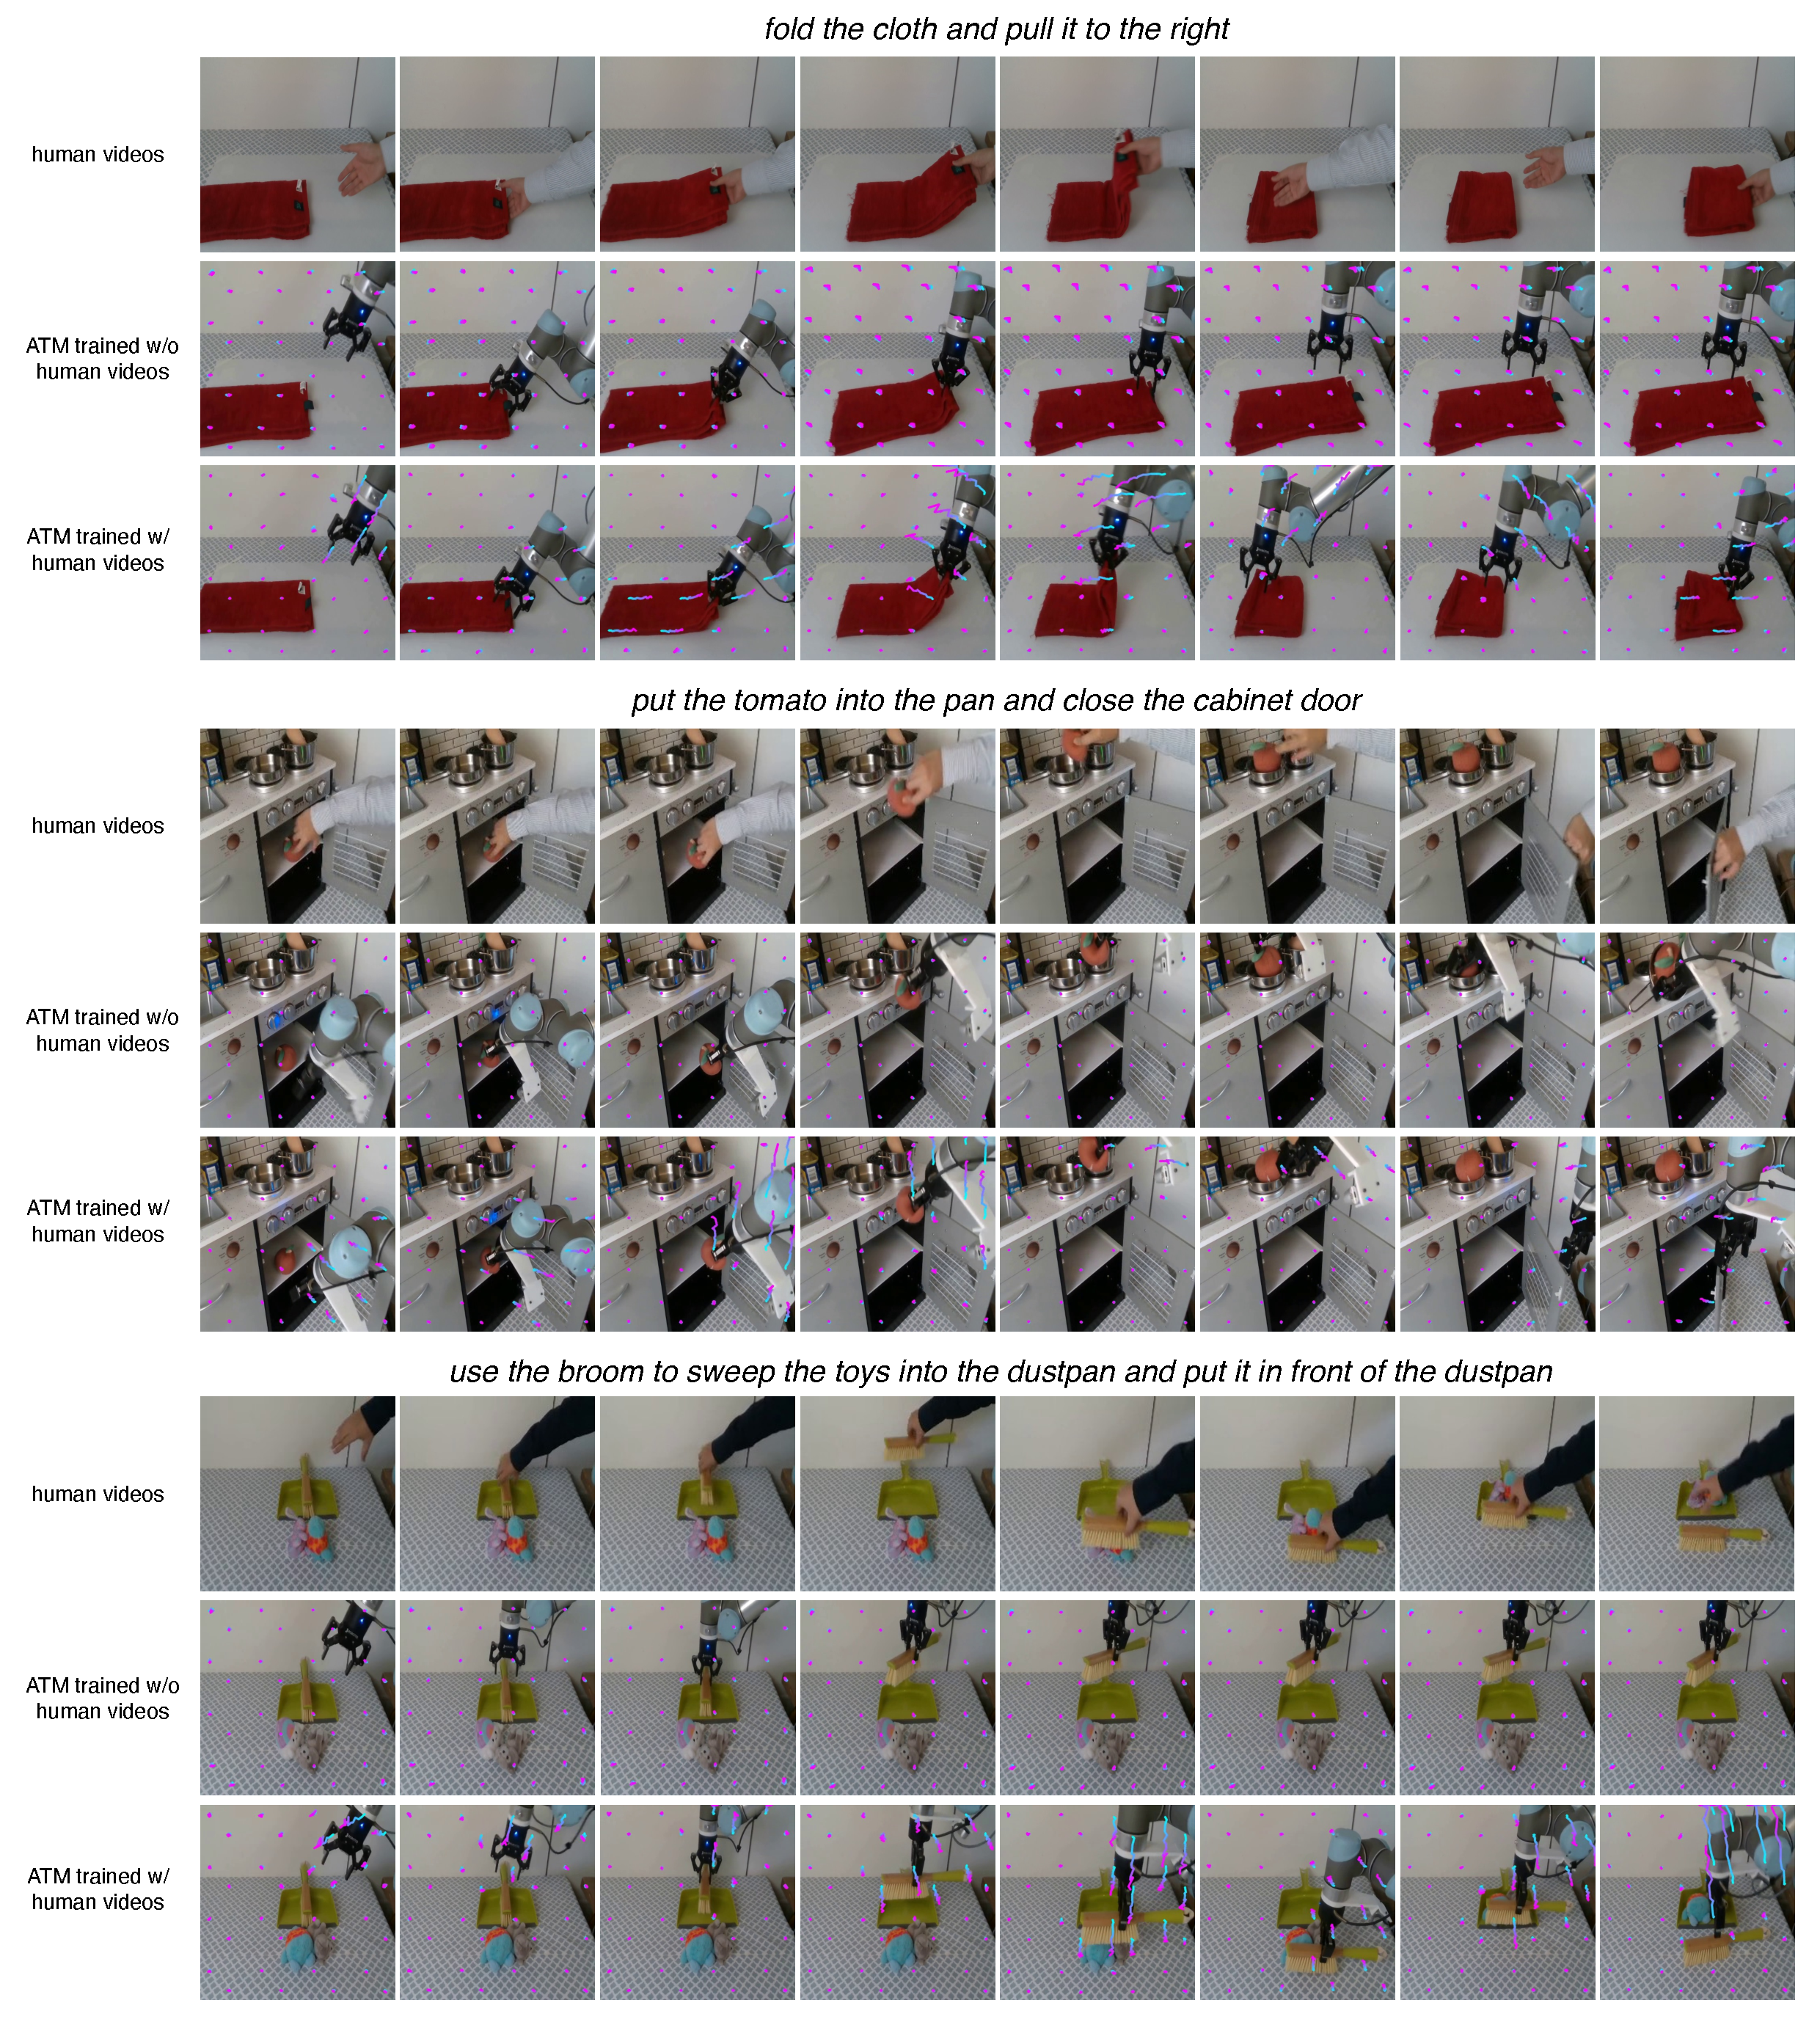
\includegraphics[width=\linewidth]{fig/human_video_supp_3task.pdf}
    \caption{通过人类数据和没有人类数据训练的人类演示和ATM策略的推广视频. 我们可以看到ATM能够利用域外视频,即人类视频,产生更精确的轨道,从而提高策略性能.}
    \label{fig:human_video_supp}
\end{figure*}


\section{实施细节}
\subsection{策略架构}~\label{sec:app:policy-arch}
我们包括ViT-T的更详细视图~\cite{liu2023libero, kim2021vilt} 在图中使用的实验~\ref{fig:arch-appendix}我们的策略中输入是多个视图中的暂时堆叠图像集 $o_t \in \mathbb{R}^{V\times T \times C\times H\times W}$子,子,子,子,子,子,子,子,子,子,子,子,子,子,子,子,子,子,子,子,子,子,子,子,子,子,子,子,子,子,子,子,子,子,子,子,子,子,子,子,子,子,子,子,子,子,子,子,子,子,子,子,子,子,子,子,子,子,子,子,子,子,子,子,子,子,子,子,子,子,子,子,子,子,子,子,子,子,子,子,子,子,子,子,子 $p_t \in \mathbb{R}^{D_p}$为了处理这些输入,ViT-T由三个阶段组成: \\

空间编码:我们在每一步都编码所有模式.首先我们利用结的轨迹 Transformer为所有人提出一套轨道. $V$ 的 $o_t$然后我们将每个模式进行投影,使用特定模式的编码器, $\mathbb{R}^D$通过使用共享学习模式代币和特定模式的位置嵌入,每个模式代币嵌入.然后我们将代币连接到所有模式和视图中,使用学习空间 CLS代币,并对序列进行自我注意.我们将空间 CLS代币作为表示. \\

时间解码:我们将编码的模式在时间阶段进行处理,首先将每一个时间阶段的自觉感知投影到同一共享嵌入空间中. $\mathbb{R}^D$然后我们将编码的自觉感知,空间CLS标记和学习的行动CLS标记交叉时间步骤, \\

行动头:我们独立处理每个时间步骤的输出,并使用MLP进行参数化. \\

\subsection{通过点选进行有效训练}\label{sec:app:track-filter}
我们采用一个论法来过背景中的静态点,然后使用现行跟踪模型来生成大运动点的相应轨迹.~\ref{fig:filtering}.


\subsection{培训细节}~\label{sec:app:train-detail}
我们列出了轨迹 Transformer的训练超参数和轨迹引导策略在表中~\ref{tab:tt-hyperparameter} 其他 \ref{tab:policy-hyperparameter}我们将所有模型都训练用4个A100GPU,

我们训练了轨迹 Transformer,使用CoTracker生成的地面真相轨道.~\cite{karaev2023cotracker} 我们不包括轨迹 Transformer的框架堆,以避免因果混乱~\cite{wen2022primenet}. 

我们通过使用LIBERO提供的专家示范培训策略,~\cite{liu2023libero}由于行为克隆的验证损失并不总是可靠的,


\end{document}


